
\subject{City location descriptions for ATS}
\title{Company\!/Facility Directory}
\subtitle{Preview Edition}

\hypersetup{
	pdfsubject={City location descriptions for ATS},
	pdftitle={Company/Facility Directory (Preview)},
}

\begin{document}

\maketitle

\vspace{5mm}
\section*{Preamble}

{
\justifying

The Company/Facility Directory (C/FD) is designed to assist those who like driving in American Truck Simulator without the help of simulated GPS navigation.

This \textbf{early preview edition} only contains those eight states for which the C/FD is already more or less complete.
Some \emph{in}complete additional content for other states is available separately as a supplement.

%This project is quite new and I don't really know yet where I'm going with it.
%Right now, the content structure is very similar to that of the wiki I used to upload these location descriptions to prior to February 2023.
%But it's not necessarily useful for it to stay that way.
%The idea is for the C/FD to be printable on paper---unlike the wiki, which was optimized to be viewed on a screen.
%Trading hypertext for a fixed canvas size brings both new challenges and opportunities.

%I don't know yet how the final edition of the C/FD will be structured and collated, nor what other content besides location descriptions it will eventually contain.
%Additionally, the visual design might change significantly from this early preview edition.
%This document has been typeset with \TeX, so it would even be relatively easy to produce multiple different versions---say, one for screen viewing, another one for printing.

The final edition of the C/FD may look very different from this early preview.
Future updates will be made available on the SCS forum.
Should you find this project interesting, please join the discussion!

\centering \vspace{1ex}
\url{https://forum.scssoft.com/viewtopic.php?t=317942} \par
}

{
\centering \vspace{30mm} \footnotesize \itshape
Copyright \raisebox{.2ex}{\scriptsize\copyright} \the\year\ nautofon \par
\vspace{.4ex}
\href{https://creativecommons.org/licenses/by-nc-sa/4.0/}{CC BY-NC-SA 4.0} \par
\vspace{.4ex}
Typeset in \TeX \par
}
\thispagestyle{empty}

\tableofcontents
\thispagestyle{empty}

\chapter{Arizona}
\ChapterForState{AZ}{Arizona}

\City{Camp Verde}

\begin{LocationList}

\Location{Mon Coeur}
Northeast of downtown Camp Verde.

\Location{Sell Goods}
North in downtown Camp Verde.

\Location{Shop Town}
Southwest in downtown Camp Verde.

\Location{Sunshine Crops}
On Wilshire~Blvd, off \AZ{260} west of \I{17} \Exit{287}.

\Location{\TruckStop \Gas \Rest}
On \AZ{260}, west of \I{17} \Exit{287}.

\end{LocationList}

\City{Clifton}

\begin{LocationList}

\Location{Coastline Mining}
Outside \Town{Morenci} by \US{191}.

\Location{Gallon Oil \UndergroundTank \Gas}
At the Gallon Oil gas station on \US{191}.

\Location{Tidbit}
On \US{191}.

\Location{\TruckService \Service \Rest}
On \US{191}.

\end{LocationList}

\penalty -350  % \pagebreak[3] == \penalty -301, which is not quite enough
\City{Flagstaff}

\begin{LocationList}

\Location{Bitumen}
On Cherry~Ave at Beaver~St, off \US{180} Humphreys~St.

\Location{Eddy's}
On Aspen~St, between Leroux~St and Verde~St.

\Location{Gallon Oil \UndergroundTank \Gas \Rest}
At the Gallon Oil truck stop off \I{40}[Bus] to the south.

\Location{\GarageHQ \Garage}
On Cherry~Ave at Leroux~St.

\Location{HMS Machinery}
On \AZ{66} in \Town{Seligman}[,] west of Flagstaff off \I{40} \Exit{121}.

\Location{International \TruckDealer \Dealer \Rest \Service}
On Verde~St at Cherry~Ave.

\Location{Plaster \& Sons}
On \US{180}, just northwest of Flagstaff.

\Location{Sell Goods}
On Aspen~St at Verde~St.

\Location{Voltison Motors}
On Leroux~St at Aspen~St.

\Location{Wallbert}
On Cherry~Ave at Leroux~St.

\end{LocationList}

\City{Grand Canyon Village}

\begin{LocationList}

\Location{Bitumen depot}
On the southern street leading to Canyon View off \AZ{64}.
% Inexplicably, the "Center Rd" street name sign was removed some time between 1.36 and 1.46.

\Location{Bitumen garage}
In \Town{Valle} on \AZ{64}.

\Location{Bitumen roadworks}
At Canyon View off \AZ{64}.

\Location{Gallon Oil \UndergroundTank \Gas}
On the southern street leading to Canyon View off \AZ{64}.

\Location{Tidbit}
On \AZ{64}.

\end{LocationList}

\GasRestNote{The closest truck stop with a rest area is located in \Town{Cameron} at the intersection of \AZ{64} and \US{89}.}

\City{Holbrook}

\begin{LocationList}

\Location{Bushnell Farms}
On St~Anselm~Rd at Chambers~Rd, off \US{191} to the east.
From~\I{40}, take \Exit{359} and head south, then turn right.
%From~\I{40} \Exit{333} head north, then turn right.

\Location{Coastline Mining}
On Quarry~Rd off \US{191}, south of \I{40} \Exit{333}.

\Location{Gallon Oil \UndergroundTank \Gas}
At the Gallon Oil gas station on Buffalo~St, west of \US{180} \AZ{77} Navajo~Blvd.

\Location{Plaster \& Sons}
On Florida~St, west of \US{180} \AZ{77} Navajo~Blvd.

\Location{Rail Export}
On St~Anselm~Rd off \US{191}, south of \I{40} \Exit{333}.

\Location{Tidbit}
On Hopi~Dr, west of \US{180} \AZ{77} Navajo~Blvd.

\Location{\TruckStop \Gas \Rest}
By \I{40} \Exit{286}.

\end{LocationList}

\City{Kayenta}

\begin{LocationList}

\Location{Coastline Mining}
Accessed from \US{191}, 5~miles south of \US{160}.

\Location{Gallon Oil \UndergroundTank \Gas \Rest}
South of \US{160} at \US{163}.

\Location{Sunshine Crops}
South of \US{160} at \US{163}.

\Location{Tidbit}
On \US{163}.

\end{LocationList}

\City{Kingman}

\begin{figure}[b!]
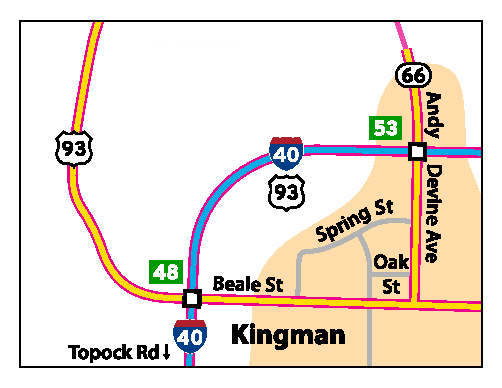
\includegraphics[scale=0.77]{cities/arizona/kingman}
\centering\caption{Street name map of Kingman, Arizona}
\end{figure}

\begin{LocationList}

\Location{Bitumen depot}
On Spring~St, off Andy Devine~Ave.

\Location{Bitumen roadworks}
On \AZ{66}, halfway between Kingman and \Town{Peach Springs}[.]

\Location{\GasStation \Gas}
On Spring~St, off Andy Devine~Ave.

\Location{HMS Machinery}
On Topock~Rd, off \I{40} \Exit{1}.

\Location{Plaster \& Sons \SpecialTransport}
On Oak~St, off Andy Devine~Ave.

\Location{Sell Goods}
On Spring~St at Beale~St.

\Location{\TruckService \Service \Rest}
On Andy Devine~Ave at Oak~St.

\Location{Wallbert \Multiple}
On \AZ{66} Andy Devine~Ave.
%There are two Wallbert facilities here.
A food warehouse is on the west side of the street and a non-food market on the east side.

\end{LocationList}

\City{Nogales}

\begin{LocationList}

\Location{Apade}
On Mariposa~Rd, off \I{19} \Exit{4}.

\Location{Coastline Mining}
On Ruby~Rd, off \I{19} \Exit{12}.

\Location{Gallon Oil \UndergroundTank \Gas}
At the Gallon Oil gas station on Mariposa~Rd, off \I{19} \Exit{4}.

\Location{Plaster \& Sons building foundation}
On Mariposa~Rd, off \I{19} \Exit{4}.

\Location{Plaster \& Sons warehouse}
On Crawford~St at Mariposa~Rd.

\Location{Sell Goods}
On Mariposa~Rd, off \I{19} \Exit{4}.

\Location{Shop Town}
On Mariposa~Rd, off \I{19} \Exit{4}.

\Location{Sunshine Crops}
On Mariposa~Rd, off \I{19} \Exit{4} to the east.

\Location{\TruckStop \Gas \Rest}
On Crawford~St at Terrace~Ave.

\end{LocationList}

\City{Page}

\begin{LocationList}

\Location{Bitumen}
On Coppermine~Rd.

\Location{Gallon Oil}
By \AZ{98} just outside Page.

\Location{HMS Machinery}
On Lake Powell~Blvd, north in Page.

\Location{\TruckService \Service \Rest}
On \AZ{98}, east in Page.

\Location{\TruckStop \Gas \Rest}
On Lake Powell~Blvd, north in Page.

\Location{Wallbert food warehouse}
On Lake Powell~Blvd at \AZ{98} Navajo~Dr.

\Location{Wallbert non-food market}
On \AZ{98} Navajo~Dr.

\end{LocationList}

\City{Phoenix}

\begin{LocationList}

\Location{42 Print}
On Indian School~Rd at 33rd~Ave, off \I{10} \Exit{141} to the north.

\Location{Bitumen}
East of 7th~St, off \I{17} \Exit{201} to the east.

\Location{Bushnell Farms}
Off \AZ{85} 35~miles south of Phoenix, by \I{8} \Exit{115}.

\Location{Charged}
On University~Dr at Buckeye~Rd, southwest of \I{10} \Exit{149}.
%On University~Dr at Buckeye~Rd, off \I{10} \Exit{149} to the southwest.

\Location{Chemso}
On Buckeye~Rd, off \I{17} \AZ{85} \Exit{199} to the west.

\Location{Coastline Mining}
On 19th~Ave off Buckeye~Rd, southeast of \I{17} \AZ{85} \Exit{199}.
%On 19th~Ave south of Buckeye~Rd, off \I{17} \AZ{85} \Exit{199} to the east.

\Location{Enterpriser}
On 32nd~Ave at Catalina~Dr, off \I{17} \Exit{201} to the west.

\Location{Gallon Oil \UndergroundTank \Gas}
At the Gallon Oil gas station on Thomas~Rd, off \I{17} \Exit{201} to the west.

\Location{\GarageHQ \Garage}
On Indian School~Rd at 35th~Ave, off \I{10} \Exit{141} to the north.

\Location{Kenworth \TruckDealer \Dealer \Rest \Service}
On Indian School~Rd at 33rd~Ave, off \I{10} \Exit{141} to the north.

\Location{Phoenix Freight \Rest \SpecialTransport}
On Magnolia~St at University~Dr, just south of Sky Harbor airport off \I{10} \Exit{149}.

\Location{Plaster \& Sons}
On Thomas~Rd in northeast Phoenix, off \AZ{51} \Exit{2} to the west.

\Location{\RecruitmentAgency \Recruitment}
On 32nd~Ave, off \I{17} \Exit{201} to the west.

\Location{Sell Goods}
On 20th~St off Buckeye~Rd, northeast of \I{17} \AZ{85} \Exit{199}.
%On 20th~St north of Buckeye~Rd, off \I{17} \AZ{85} \Exit{199} to the east.

\Location{Starbridge}
On Buckeye~Rd, off \I{17} \AZ{85} \Exit{199} to the east.

\Location{Venture}
On Thomas~Rd at 33rd~Ave, off \I{17} \Exit{201} to the west.

\end{LocationList}

\City{San Simon}

\begin{LocationList}

\Location{Darchelle Uzau}
On Apache Pass~Rd, off \I{10} \Exit{337} west of San Simon.

\Location{Gallon Oil \UndergroundTank \Gas \Rest}
At the Gallon Oil truck stop on \I{10}[Bus] in San Simon.

\Location{Sunshine Crops farm}
On Portal~Rd off \I{10} \Exit{382}, 15~miles south of San Simon.

\Location{Sunshine Crops garage}
On \I{10}[Bus] in San Simon.

\end{LocationList}

\City{Show Low}

\begin{LocationList}

\Location{\RestArea \Rest}
On Rainbow Lake~Rd, off \AZ{260} in Pinetop--Lakeside.

\Location{Sell Goods}
By Owens~St, off \AZ{260} White Mountain~Rd.

\Location{Voltison Motors}
On \US{60} \AZ{77} Deuce of Clubs.

\Location{Wallbert}
On Club Lake~Rd at Scott Ranch~Rd, off \AZ{260} White Mountain~Rd.
%By Scott Ranch~Rd, off \AZ{260} White Mountain Rd.

\end{LocationList}

\GasRestNote{The closest truck stop with a gas station is located in \CityRef{Holbrook} to the north.}
%\GasRestNote{The closest gas station is located in \CityRef{Holbrook} to the north.}

\City{Sierra Vista}

\begin{LocationList}

\Location{Bitumen}
On Fry~Blvd at Lenzer~Ave.

\Location{Coastline Mining}
Off \AZ{92} to the east at Buffalo Soldier~Trl.

\Location{Eddy's}
On \AZ{90} at Fry~Blvd.

\Location{\RecruitmentAgency \Recruitment}
On Fry~Blvd.

\Location{\TruckStop \Gas \Rest}
On Commerce~Dr, by \I{10} \Exit{302}.

\Location{Wallbert}
On \AZ{92}.

\end{LocationList}

\pagebreak[3]
\City{Tucson}

\begin{LocationList}

\Location{Bitumen garage}
On 15th~St.

\Location{Bitumen roadworks}
On Congress~St at \q{A} Mountain~Rd.

\Location{Charged}
On Valencia~Rd at 10th~Ave.

\Location{Gallon Oil}
On 6th~Ave at 16th~St.

\Location{\GarageHQ \Garage}
On Congress~St, between 7th~Ave and 10th~Ave.

\Location{\GasStation \Gas}
On 6th~Ave at 16th~St.

\Location{Plaster \& Sons}
On 16th~St.

\Location{\RecruitmentAgency \Recruitment}
On Congress~St, between 7th~Ave and 10th~Ave.

\Location{Volvo \TruckDealer \Dealer \Rest \Service}
On 6th~Ave at \I{10} \Exit{261}.

\Location{Wallbert food warehouse}
On 14th~St at Granada~Ave.

\Location{Wallbert non-food market}
On 6th~Ave at \I{10} \Exit{261}.

\end{LocationList}

\begin{figure}[hp]
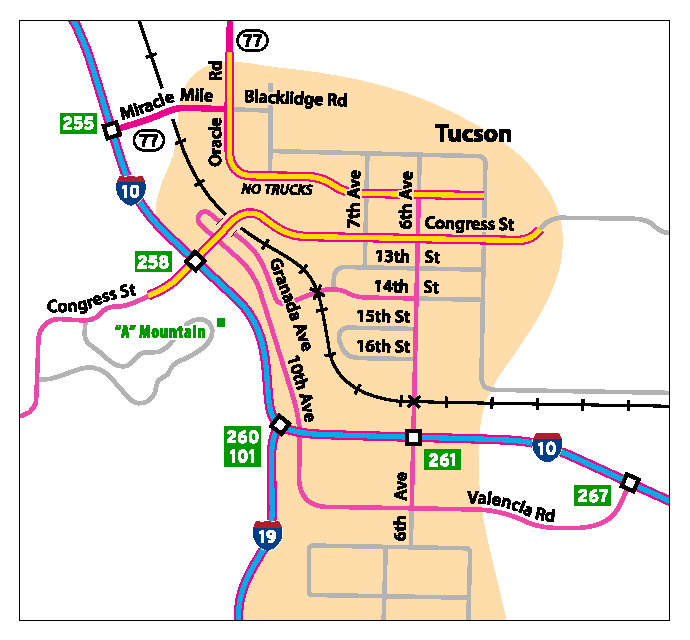
\includegraphics[scale=0.88]{cities/arizona/tucson}
\centering\caption{Street name map of Tucson, Arizona}
\end{figure}
\pagebreak[4]

\City{Yuma}

\begin{LocationList}

\Location{Eddy's}
North of 16th~St in downtown Yuma.

\Location{\GarageHQ \Garage}
On 16th~Ave east of \US{95}.

\Location{Peterbilt \TruckDealer \Dealer \Rest \Service}
On 16th~Ave east of \US{95}.

\Location{Plaster \& Sons}
By Arizona~Ave south of 16th~St.

\Location{Rail Export}
North of 16th~St in downtown Yuma.

\Location{Sunshine Crops}
On \US{95}, north of \I{8} \Exit{2}.

\Location{\TruckStop \Gas \Rest \Weigh}
On 16th~Ave at \US{95}.

\Location{Voltison Motors}
On Arizona~Ave north of 16th~St.

\Location{Wallbert \SpecialTransport}
On Arizona~Ave south of 16th~St.

\end{LocationList}

\begin{figure}[hp]
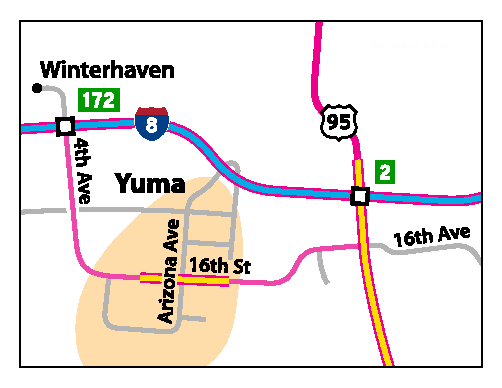
\includegraphics[scale=0.77]{cities/arizona/yuma}
\centering\caption{Street name map of Yuma, Arizona}
\end{figure}



\chapter{Colorado}
\City{Alamosa}

\begin{LocationList}

\Location{AI Automotive}
On Craft~Dr, south of \US{160} \US{285} Main~St.

\Location{Avalanche Steel}
Off \US{160} to the north at the truck stop.

\Location{Bitumen}
On \US{160} 6th~St, east of \US{285}.

\Location{Drake Car Dealer}
On Craft~Dr, south of \US{160} \US{285} Main~St.

\Location{\GarageHQ \Garage}
Off \US{160} to the south at the truck stop.

\Location{HMS Machinery}
Off \US{160} to the north at the truck stop.

\Location{\RecruitmentAgency \Recruitment}
On \US{160} 6th~St.

\Location{Steeler}
In \Town{Monte Vista} on \US{285}.

\Location{\TruckStop \Gas \Rest \Service}
On \US{160}, east in Alamosa.

\Location{Wallbert}
On \US{160} \US{285} Main~St at Craft~Dr.

\Location{Western Star \TruckDealer \Dealer \Rest \Service}
On Craft~Dr, south of \US{160} \US{285} Main~St.

\end{LocationList}

\City{Burlington}

\begin{LocationList}

\Location{Bushnell Farms}
By \US{385}, just south of the truck stop.

\Location{Drake Car Dealer}
On \US{385} Rose~Ave.

\Location{NAMIQ}
By \US{385} at the railroad crossing.

\Location{Phoenix \UndergroundTank \Gas \Rest \Service \Weigh}
At the Phoenix truck stop on \US{385} by \I{70} \Exit{437}.

\Location{Sunshine Crops farm \SpecialTransport}
Off \US{385} in northeastern Burlington.

\Location{Sunshine Crops garage}
On \US{385} Lincoln~St.

\end{LocationList}

\City{Colorado Springs}

\begin{LocationList}

\Location{42 Print}
On Cascade~Ave north of Fillmore~St, off \I{25} \Exit{145} to the east.

\Location{Drake Car Dealer}
On \CO{21} Powers~Blvd north of \US{24}.
Use \I{25} \Exit{139}.

\Location{\GarageHQ \Garage}
Off Cascade~Ave north of Fillmore~St.
Use \I{25} \Exit{145}.

\Location{Mack \TruckDealer \Dealer \Rest \Service}
By Cascade~Ave north of Fillmore~St.
Use \I{25} \Exit{145}.

\Location{NAF \UndergroundTank \Gas \Rest}
At the NAF gas station on Aeroplaza~Dr by \US{24} Powers~Blvd.
Use~\I{25} \Exit{139}.

\Location{NAMIQ \Multiple \Rest}
Accessed from \CO{67}, 15~miles south of \US{24} through \Town{Divide}[.]
%There are two NAMIQ facilities here:
A warehouse with a rest area is accessed from the north and a quarry is further south.

\Location{Sell Goods}
By Aeroplaza~Dr, off \US{24} Powers~Blvd to the east.
Use~\I{25} \Exit{139}.

% From ATS IRL map:
%On Vapor~Trl between Fountain~Blvd and Aeroplaza~Dr, off \US{24} \CO{21} Powers~Blvd to the east.
%Use \I{25} \Exit{139}.

\Location{Wallbert market}
On Moreno~Ave at 8th~St, south of \US{24} off \I{25} \Exit{141}.

% From ATS IRL map:
%On Moreno~Ave at 8th~St, south of \US{24} Cimarron~St off \I{25} \Exit{141}.

\Location{Wallbert warehouse}
Off \US{24} Powers~Blvd to the east.
Use \I{25} \Exit{139}.

% From ATS IRL map:
%On Newport~Rd between Fountain~Blvd and Aeroplaza~Dr, off \US{24} \CO{21} Powers~Blvd to the east.
%Use \I{25} \Exit{139}.

\end{LocationList}

\City{Denver}

\begin{LocationList}

\Location{Bitumen}
On the westbound ramp at \I{70} \Exit{232} for \US{40}.

\Location{Denver Air Cargo}
Off Jackson Gap~St at the airport.
Use \I{70} \Exits{284}{285}.

\Location{\GarageHQ \Garage}
On Josephine~St, off \I{70} \Exit{275}.

\Location{Haulett \UndergroundTank \Gas \Rest \Weigh}
At the Haulett truck stop on 32nd~Ave in \Town{Aurora}[,] off \I{70} \Exit{285}.

\Location{International \TruckDealer \Dealer \Rest \Service}
On 32nd~Ave in \Town{Aurora}[,] off \I{70} \Exit{285}.

\Location{Rail Export \SpecialTransport}
On York~St, off \I{70} \Exit{275}.

\Location{\RecruitmentAgency \Recruitment}
By 32nd~Ave in \Town{Aurora}[,] off \I{70} \Exit{283}.

\Location{Sell Goods}
On 32nd~Ave in \Town{Aurora}[,] off \I{70} \Exit{285}.

\Location{USBB}
On 40th~Ave at York~St, off \I{70} \Exit{275}.

\Location{Ultimus \SpecialTransport}
On the tarmac past the Air Cargo terminal off Jackson Gap~St.
Use~\I{70} \Exits{284}{285}.

\Location{Vitas Power}
Accessed from \CO{71}, 10~miles north of \Town{Limon}[.]

\Location{Wallbert market}
On \CO{30} Hampden~Ave at Locust~St in southern Denver, off \I{25} \Exit{201}.

\Location{Wallbert warehouse}
On 32nd~Ave in Aurora, off \I{70} \Exit{285}.

\end{LocationList}

\City{Durango}

\begin{LocationList}

\Location{Drake Car Dealer}
On Dominguez~Dr, northeast of \US{160} \US{550} Camino Del Rio.

\Location{\GasStation \Gas \Rest}
On Dominguez~Dr, northeast of \US{160} \US{550} Camino Del Rio.

\Location{Home Store}
On \US{160} \US{550} Camino Del Rio at Dominguez~Dr.

\Location{Shop Town}
On \US{160} \US{550} Camino Del Rio at Dominguez~Dr.

\Location{Tidbit}
On \US{550} Camino Del Rio at 9th~St.

\Location{\TruckService \Service \Rest}
On Dominguez~Dr, northeast of \US{160} \US{550} Camino Del Rio.

\end{LocationList}

\City{Fort Collins}

\CityDisclaimer{ATS IRL Map}

\begin{LocationList}

\Location{Avalanche Steel}
On \US{287} College~Ave, north in Fort Collins.

\Location{Bitumen}
In \Town{Loveland} on \US{287} Lincoln~Ave, north of \US{34}.

\Location{Bushnell Farms \Multiple}
Off \US{287} to the southwest just north of Fort Collins.
%There are two Bushnell Farms facilities here:
A livestock auction site is next to the highway, and a farm is further down the highway and off to the left.%
\textsuperscript{\scriptsize $\dagger$}

\Location{Farmer's Barn}
On Vine~Dr, off \US{287} College~Ave to the east.
From \CO{14}, turn~right.

\Location{Freightliner \TruckDealer \Dealer \Rest \Service}
In \Town{Loveland} by \US{287} north of \US{34}.

\Location{\GarageHQ \Garage}
On Vine~Dr, off \US{287} College~Ave to the east.

\Location{\GasStation \Gas}
On \US{287} College~Ave at Vine~Dr, north of \CO{14}.

\Location{Home Store}
On Lemay~Ave at Vine~Dr, north of \CO{14} Mulberry~St.

\Location{\RecruitmentAgency \Recruitment}
In \Town{Loveland} on \US{287} north of \US{34}.

\Location{\RestArea \Rest}
On Lemay~Ave north of \CO{14} Mulberry~St.

\Location{Sell Goods}
In \Town{Loveland} on \US{287} north of \US{34}.

\Location{Sunshine Crops}
Accessed from \CO{1} Terry Lake~Rd, off \US{287} to the northeast just north of Fort Collins.

\Location{Wallbert}
On Lemay~Ave at \CO{14} Mulberry~St.

\end{LocationList}

\City{Grand Junction}

\begin{LocationList}

\Location{Bushnell Farms}
On \CO{139} in \Town{Loma}[,] off \I{70} \Exit{15}.

\Location{Drake Car Dealer}
On \US{50}, southeast of \I{70} \Exit{26}.

\Location{Haulett \UndergroundTank \Gas \Rest \Weigh}
At the Haulett truck stop by \I{70} \Exit{19}.

\Location{Home Store}
Off \US{6} \US{50} to the northeast at Donut Planet.

\Location{Sell Goods}
Off \US{6} opposite the Driverse truck stop by \I{70} \Exit{26}.

\Location{Volvo \TruckDealer \Dealer \Rest \Service}
Past the Haulett truck stop by \I{70} \Exit{19}.

\Location{Wallbert}
Off \US{6} \US{50} to the northeast at Dream Burger.

\end{LocationList}

\City{Lamar}

\begin{LocationList}

\Location{Bushnell Farms}
By \US{50} at \US{287}, west of Lamar.
Accessed from the frontage road to the south.

\Location{Farmer's Barn}
On Maple~St, off \US{50} \US{287} Main~St to the east.

\Location{\GarageHQ \Garage}
Off \US{50} \US{287} to the northeast, between Lamar and the weigh station to the west.

\Location{Phoenix \UndergroundTank \Gas \Rest}
At the Phoenix truck stop on Maple~St at \US{50} \US{287} Main~St.

\Location{Sell Goods}
Off \US{50} \US{287} to the northeast, between Lamar and the weigh station to the west.

\Location{Sunshine Crops}
Southeast of Lamar, past the Wallbert off \US{50} \US{385}.

\Location{\TruckStop \Gas \Rest \Weigh}
On Ave~Colonia at \US{50} \US{287} Main~St.

\Location{Wallbert}
By \US{50} \US{385} Olive~St.

\end{LocationList}

\penalty -350  % \pagebreak[3] == \penalty -301, which is not quite enough
\City{Montrose}

\begin{LocationList}

\Location{Apade}
On \US{50} Townsend~Ave.

\Location{Deepgrove}
On 6530~Rd off \US{50} San Juan~Ave.

\Location{Drake Car Dealer}
On Grand~Ave, west of \US{50} Townsend~Ave.

\Location{Enterpriser}
Off \US{550} Townsend~Ave to the west opposite Donut Planet.

\Location{Farmer's Barn}
On \US{550} Townsend~Ave.

\Location{\GarageHQ \Garage}
Off \US{50} Townsend~Ave to the west.

\Location{NAMIQ}
At \Town{Camp Bird}[,] accessed from \US{550} outside \Town{Ouray}[,] 30~miles south of Montrose.

\Location{Peterbilt \TruckDealer \Dealer \Rest \Service}
On \US{50} San Juan~Ave at 6530~Rd.

\Location{\TruckStop \Gas \Rest \Weigh}
On \US{50} Townsend~Ave.

\end{LocationList}

\City{Pueblo}

\begin{LocationList}

\Location{Avalanche Steel}
On Northern~Ave, off \I{25} \Exit{97}.

\Location{Deepgrove}
On Northern~Ave, off \I{25} \Exit{97}.

\Location{Drake Car Dealer}
On \US{50}, off \I{25} \Exit{101}.

\Location{Gallon Oil \UndergroundTank \Gas \Rest \Service \Weigh}
At the Phoenix truck stop on Drew Dix~Pkwy, off \I{25} \Exit{104}.

\Location{HMS Machinery}
On Elizabeth~St, between Drew Dix~Pkwy and \US{50} off~\I{25} \Exit{101}.

\Location{Home Store}
On \US{50}, off \I{25} \Exit{101}.

\Location{Kenworth \TruckDealer \Dealer \Rest \Service}
On \US{50}, off \I{25} \Exit{101}.

\Location{Vitas Power construction site}
By \US{350}, halfway between \Town{La Junta} and \Town{Trinidad}[.]

\Location{Vitas Power factory}
Off \I{25} \Exit{91}.

\Location{Wallbert}
By \CO{47}, off \I{25} \Exit{101}.

\end{LocationList}

\City{Rangely}

\begin{LocationList}

\Location{Avalanche Steel}
Off \CO{64}.

\Location{Drake Car Dealer}
On \CO{64}.

\Location{Gallon Oil \Multiple}
Accessed from \CO{64} just north of Rangely.
%There are two Gallon Oil facilities here:
An oil drilling site is to the right and a storage facility is to the left.%
\textsuperscript{\scriptsize $\dagger$}

\Location{Tidbit}
By \CO{64}.

\Location{\GasStation \Gas \Rest}
In \Town{Dinosaur} on \US{40}.

\end{LocationList}

\penalty -500  % \pagebreak[3] == \penalty -301, which is not quite enough
\City{Steamboat Springs}

\begin{LocationList}

\Location{Deepgrove}
Accessed from \CO{131}, 20~miles south of Steamboat Springs.

\Location{\GarageHQ \Garage}
On Elk River~Rd, north of \US{40} Lincoln~Ave.

\Location{\GasStation \Gas}
On Elk River~Rd at \US{40} Lincoln~Ave.

\Location{HMS Machinery}
Accessed from \CO{13}, 10~miles south of \Town{Craig}[.]

\Location{Plaster \& Sons}
On Mt Werner~Rd, north of \US{40}.

\Location{\RestArea \Rest}
Next to the Wallbert off Mt Werner~Rd, north of \US{40}.

\Location{Sell Goods}
On 13th~St, off \US{40} Lincoln~Ave to the south.

\Location{\TruckService \Service}
On 13th~St, off \US{40} Lincoln~Ave to the south.

\Location{Voltison Motors}
On \US{40} Lincoln~Ave at Elk River~Rd.

\Location{Wallbert}
Off Mt Werner~Rd, north of \US{40}.

\end{LocationList}

\City{Sterling}

\begin{LocationList}

\Location{Bushnell Farms \Rest}
Accessed from \US{34}, 10~miles west of \US{385} through \Town{Wray}[.]
%A rest area is on the soft shoulder by the highway.

\Location{Farmer's Barn}
In the industrial area south of the railroad tracks.
From \US{6}, take~Main~St south and turn left at the end.

\Location{\GarageHQ \Garage}
In the industrial area south of the railroad tracks.
From \US{6}, take~Main~St south and turn left at the end.

\Location{Global Mills}
Off \US{6}, west in Sterling.

\Location{Home Store}
On \CO{14} Main~St.

\Location{Shop Town}
On \CO{14} Main~St.

\Location{Steeler \SpecialTransport}
In the industrial area south of the railroad tracks.
From \US{6}, take~Main~St south and turn left at the end.

\Location{Sunshine Crops}
Accessed from \US{385}, 25~miles south of \Town{Julesburg} off \I{76} \Exit{180}.

\Location{\TruckStop \Gas \Rest \Weigh}
On \US{6} southeast of \I{76} \Exit{125}.

\end{LocationList}



\vspace{2em}\footnoterule
{\footnotesize \noindent External sources used for the state of Colorado:
\begin{description}[
	style=nextline,
	leftmargin=1.1em,
	labelsep=0pt,
	%itemsep=0pt,
	%topsep=0pt,
	parsep=0pt,
	%listparindent=\parindent,
	font=\normalfont,
]

\item[$\ast$]
ATS IRL Map by \textit{Bedavd:}
\hyperref[city:Fort Collins]{Fort Collins}
\url{https://forum.scssoft.com/viewtopic.php?t=285700}

\item[$\dagger$]
Slippy Map for ATS by \textit{truckermudgeon:}
\hyperref[city:Fort Collins]{Fort Collins},
\hyperref[city:Rangely]{Rangely}
\url{https://forum.scssoft.com/viewtopic.php?t=318267}

\end{description}
}


\chapter{Idaho}
\ChapterForState{ID}{Idaho}

\City{Boise}

\begin{LocationList}

\Location{Deepgrove \SpecialTransport}
On the south side of Federal~Way, off \ID{21} Gowen~Rd.
From \I{84} \Exit{57} turn north, then west.

\Location{Electravolt}
On Technology~Way off \ID{21} Gowen~Rd, east in Boise.

\Location{Enterpriser}
On Gowen~Rd.
From \I{84} \Exit{57} follow signs for Gowen Field.

\Location{Farmer's Barn}
On the east side of \ID{55} Eagle~Rd, by the railroad crossing.

\Location{\GarageHQ \Garage}
On Gowen~Rd. From \I{84} \Exit{57} follow signs for Gowen Field.

\Location{International \TruckDealer \Dealer \Rest \Service}
Between Gowen~Rd and Broadway~Ave, south in Boise.

\Location{Olthon Homes}
On Federal~Way off \ID{21} Gowen~Rd.
From \I{84} \Exit{57} turn north, then west.

\Location{Plaster \& Sons building construction}
Between \US{20} Front~St and \US{20} Myrtle~St in downtown Boise.

\Location{Plaster \& Sons house construction}
Accessed from Island Woods~Dr, off \ID{55} Eagle~Rd to the west.

\Location{\RecruitmentAgency \Recruitment}
Off Broadway~Ave opposite the truck stop.

\Location{\TruckStop \Gas \Rest \Service \Weigh}
On Broadway~Ave by \I{84} \Exit{54}.

\end{LocationList}

\City{Coeur d'Alene}

\begin{LocationList}

\Location{Avalanche Steel}
Off \I{90} \Exit{11} to the north.

\Location{Deepgrove}
Accessed from \US{95} opposite Putnam~Rd, 40~miles south of Coeur d'Alene.

\Location{Drake Car Dealer}
By \US{95}, just north of \I{90} \Exit{12}.

\Location{\GarageHQ \Garage}
Off \I{90} \Exit{11} to the north.
Opposite the entrance to Avalanche Steel.

\Location{HMS Machinery}
On Seltice~Way, off Northwest~Blvd to the west.

\Location{Home Store}
Off \US{95}, northeast of \I{90} \Exit{12}.

\Location{Plaster \& Sons house construction}
In \Town{Fernan}[,] off \I{90} \Exit{15}.

\Location{Plaster \& Sons warehouse construction}
In the west of the commercial area north of \I{90} \Exit{11}.

\Location{\RecruitmentAgency \Recruitment}
Off \US{95}, northeast of \I{90} \Exit{12}.

\Location{Sea Horizon}
On Marina~Dr, off \US{95} south of Coeur d'Alene.

\Location{\TruckStop \Gas \Rest \Service}
On Coeur d'Alene Lake~Dr at Sherman~Ave, off \I{90} \Exit{15}.

\Location{Wallbert}
On Sherman~Ave at 15th~St, off \I{90} \Exit{15}.

\end{LocationList}

\penalty -350  % \pagebreak[3] == \penalty -301, which is not quite enough
\City{Grangeville}

\begin{LocationList}

\Location{Coastline Mining}
Off \ID{13} to the south, just east of Grangeville.

\Location{Deepgrove sawmill}
On \US{95}, just north of Grangeville.

\Location{Deepgrove timber harvest site}
Off \US{12} to the north between \Town{Kooskia} and \Town{Kamiah}[.]

\Location{Eddy's}
On \ID{13} Main~St.

\Location{Farmer's Barn}
On County~Rd, accessed from \US{95} in the north of Grangeville.

\Location{HMS Machinery}
On County~Rd, accessed from \US{95} in the north of Grangeville.

\Location{Sunshine Crops}
Off \ID{13} to the south, just east of Grangeville.

\Location{\TruckStop \Gas \Rest}
At the intersection of \US{95} and \ID{13}.

\Location{Venture}
On \ID{13}, just east of Grangeville.

\end{LocationList}

\City{Idaho Falls}

\begin{LocationList}

\Location{Apade}
Off \US{20}[Bus] Holmes~Ave to the west, just north of the \US{26} junction.
Use \I{15} \Exit{119} and \US{20} \Exit{310}.

\Location{Enterpriser}
On Sunnyside~Rd, between Holmes~Ave and Yellowstone~Ave, just southeast of downtown.

\Location{\GarageHQ \Garage \SpecialTransport}
Off \US{20}[Bus] Holmes Ave to the west.
Use \I{15} \Exit{119} and \US{20} \Exit{310}.

\Location{HMS Machinery}
By the airport, off \I{15} \Exit{119}.

\Location{Home Store}
On Holmes~Ave, between 7th~St and Sunnyside~Rd, in the southeast of Idaho Falls.

\Location{Peterbilt \TruckDealer \Dealer \Rest \Service}
By \I{15} \Exit{113}, opposite the Haulett truck stop.

\Location{Phoenix \UndergroundTank \Gas \Rest \Service \Weigh}
At the Phoenix truck stop by \I{15} \Exit{113}.

\Location{Plaster \& Sons garage}
On Yellowstone~Ave, between Broadway~St and Sunnyside~Rd, just south of downtown.

\Location{Plaster \& Sons house construction}
On Rollandet~Ave, between 7th~St and Sunnyside~Rd, in the southeast of Idaho Falls.

\Location{\RecruitmentAgency \Recruitment}
On \US{20}, off \I{15} \Exit{118}.

%\Location{Special Transport \SpecialTransport}
%By the garage, off \US{20}[Bus] Holmes~Ave to the west. Use \I{15} \Exit{119} and \US{20} \Exit{310}.

\end{LocationList}

\City{Ketchum}

\begin{LocationList}

\Location{Bitumen}
Accessed from Saddle~Rd, northwest in Ketchum.

\Location{Eddy's}
Southeast in Ketchum.

\Location{Plaster \& Sons}
In \Town{Sun Valley}[,] east of Ketchum.

\Location{Sell Goods}
Accessed from Saddle~Rd, northwest in Ketchum.

\end{LocationList}

\GasRestNote{The closest rest area is located at the junction of \ID{75} and \US{20}. A~truck stop offering gas is further south in \CityRef{Twin Falls}.}

\City{Lewiston}

\begin{LocationList}

\Location{AI Automotive}
By \US{12}, just northeast of downtown.

\Location{Avalanche Steel}
By the Page \& Price Paper plant. Accessed from \US{12} to the south, just east of downtown.

\Location{Farmer's Barn \SpecialTransport}
In the Port Districts, off \ID{128} at the Old Spiral Highway.

\Location{Page \& Price Paper}
Accessed from \US{12} to the south, just east of downtown.

\Location{Steeler}
In the Port Districts, off \ID{128} at the Old Spiral Highway.

\Location{Western Star \TruckDealer \Dealer \Gas \Rest \Service \Weigh}
At the truck stop on the joint section of \US{12} and \US{95}.

\end{LocationList}

\City{Nampa}

\begin{LocationList}

\Location{Darchelle Uzau}
On Chicken Dinner~Rd at \ID{55} Karcher~Rd, off \I{84}[Bus].
Use~\I{84} \Exit{38}.

\Location{Farmer's Barn}
On \ID{55} Karcher~Rd, off \I{84}[Bus].
Use \I{84} \Exit{38}.

\Location{Sunshine Crops}
On Can-ada~Rd at \US{20} \US{26} Chinden~Blvd, off \I{84} \Exit{38} to the north.

\Location{Wallbert}
Off Idaho Center~Blvd to the east, by \I{84} \Exit{38}.

\end{LocationList}

\GasRestNote{The closest truck stop with gas station and rest area is located in \CityRef{Boise} by \I{84} exit 54.}

\City{Pocatello}

\begin{LocationList}

\Location{Chemso}
Off \US{30} Garrett~Way, just south of \I{86} \Exit{58}.

\Location{Coastline Mining}
Accessed from Merrill~Rd, off \I{15} \Exit{47}.

\Location{Drake Car Dealer}
By McKinley~Ave, off \US{30} Gould~St to the southwest.

\Location{Plaster \& Sons}
By \I{15} \Exit{67}.
Turn north opposite the gas station, then take the next left turn.

\Location{Rail Export}
Off \US{30} Garrett~Way, south of \I{86} \Exit{58}.

\Location{Sunshine Crops \Rest}
Off \I{86} \Exit{58} to the north.

\Location{\TruckStop \Gas \Rest \Weigh}
Southwest of \I{86} \Exit{58}.

\end{LocationList}

\City{Salmon}

\begin{LocationList}

\Location{Bushnell Farms}
On \US{93}, just north of Salmon.

\Location{Coastline Mining}
Off \US{93} Main~St to the north, between the Salmon River bridge and the \ID{28} junction.

\Location{Drake Car Dealer}
On \US{93}, in the south of Salmon.

\Location{Eddy's}
North of the junction of \US{93} and \ID{28}.

\Location{Farmer's Barn}
On \ID{28}.

\Location{\GarageHQ \Garage}
Off \US{93}, in the north of Salmon.

\Location{\GasStation \Gas \Rest}
The NAF on \US{93}.

\end{LocationList}

\penalty -350  % \pagebreak[3] == \penalty -301, which is not quite enough
\City{Sandpoint}

\begin{LocationList}

\Location{Coastline Mining \Rest \Weigh}
On Baldy Mountain Road.
From \US{2} \US{95} take Schweitzer Cutoff west, then turn south at the roundabout.

\Location{Deepgrove \Multiple \Rest}
Off Baldy Mountain Road (sawmill with rest area to the south, logging site to the north).
From \US{2} \US{95} take Schweitzer Cutoff west, then turn south at the roundabout.

\Location{Farmer's Barn}
At the end of Schweitzer Cutoff, west of \US{2} \US{95}.

\Location{HMS Machinery \Rest}
On Baldy Mountain Road.
From \US{2} \US{95} take Schweitzer Cutoff west, then turn south at the roundabout.

\Location{Home Store}
On Kootenai Cutoff, east of \US{2} \US{95}.

\Location{Plaster \& Sons}
North of Schweitzer Cutoff, off \US{2} \US{95} to the west.

\Location{Shop Town}
On Larch Street, off \US{2} to the west.

\Location{\TruckStop \Gas \Rest}
At \US{2} \US{95} and Schweitzer Cutoff.

\end{LocationList}

\City{Twin Falls}

\begin{LocationList}

\Location{Coastline Mining cement plant}
On \US{30} \US{93}[Bus] Addison~Ave.

\Location{Coastline Mining storage \Weigh}
Off \US{93}, just north of the \US{30} interchange.

\Location{\GarageHQ \Garage}
On Eastland~Dr at Kimberly~Rd, in the southeast of Twin Falls.

\Location{Haulett \UndergroundTank \Gas \Rest \Service \Weigh}
At the Haulett truck stop, off \US{93} by \I{84} \Exit{173}.

\Location{Home Store}
On the east side of \US{93}[Bus] Blue Lakes~Blvd.

\Location{Mack \TruckDealer \Dealer \Rest \Service}
On Kimberly~Rd at Eastland~Dr, in the southeast of Twin Falls.

\Location{Plaster \& Sons}
On Elizabeth~Blvd at Eastland~Dr, in the east of Twin Falls.

\Location{\RecruitmentAgency \Recruitment}
On Eastland~Dr, in the east of Twin Falls.

\Location{Sunshine Crops \SpecialTransport}
On 3700~N, off \US{93} southwest of Twin Falls.

\Location{Venture}
On Orchard~Dr, southwest of downtown.

\Location{Wallbert}
On Fillmore~St, off \US{93}.

\end{LocationList}



\chapter{Montana}
\ChapterForState{MT}{Montana}

\City{Billings}

\CityDisclaimer{ATS IRL Map}

\begin{LocationList}

\Location{18 Wheels Garage}
On Frontage~Rd northwest of \I{90} \Exit{455}.

\Location{Bushnell Farms}
On Frontage~Rd northwest of \I{90} \Exit{455}.

\Location{Chemso}
On 1st~Ave, off \MT{3} 27th~St to the east.

\Location{Gallon Oil \UndergroundTank \Gas \Rest}
The Phoenix truck stop in \Town{Hardin} by \I{90} \Exit{495}.

\Location{\GarageHQ \Garage}
On Frontage~Rd northeast of \I{90} \Exit{452}.

\Location{Global Mills}
On 1st~Ave at \MT{3} 27th~St.

\Location{Home Store}
On \US{87} Main~St north of Lake Elmo~Dr.

\Location{NAMIQ}
Accessed from \US{87}, 20~miles north of Billings.

\Location{Peterbilt \TruckDealer \Dealer \Rest \Service}
On Frontage~Rd northeast of \I{90} \Exit{455}.

\Location{Sell Goods \Gas}
On Frontage~Rd northwest of \I{90} \Exit{455}.

\Location{Sweet Beets \Weigh}
On Sugar~Ave at State~Ave, off \MT{3} 27th~St to the west.

\end{LocationList}

\City{Bozeman}

\CityDisclaimer{ATS IRL Map}

\begin{LocationList}

\Location{Enterpriser}
On Frontage~Rd, off \I{90} \Exit{309} to the east.

\Location{Global Mills}
On \I{90}[Bus] 7th~Ave, north of \US{191} Main~St.

\Location{MWM}
On Griffin~Dr off 7th~Ave, northeast of \I{90} \Exit{306}.

\Location{NAMIQ \Multiple}
By \US{287} north of \Town{West Yellowstone}[.]
A quarry is located west of the highway, a talc plant is in \Town{Ennis} further on.%
\textsuperscript{\scriptsize $\dagger$}

\Location{Plaster \& Sons}
On 19th~Ave at College~St, off \US{191} Main~St to the south.

\Location{Shop Town}
On Oak~St at \I{90}[Bus] 7th~Ave, southeast of \I{90} \Exit{306}.

\Location{Starbridge}
On Frontage~Rd, off \I{90} \Exit{309} to the east.

\Location{Sunshine Crops}
By \US{191} outside \Town{Four Corners}[.]

\Location{\TruckService \Service}
On Griffin~Dr off 7th~Ave, northeast of \I{90} \Exit{306}.

\Location{\TruckStop \Gas \Rest}
In \Town{Four Corners} by \US{191}.

\Location{Walden's}
Off 7th~Ave, northwest of \I{90} \Exit{306}.

\end{LocationList}

\penalty -350  % \pagebreak[3] == \penalty -301, which is not quite enough
\City{Butte}

\CityDisclaimer{ATS IRL Map}

\begin{LocationList}

\Location{Chemso}
On Rick Jones~Way, off \I{15} \Exit{119} south of Butte.

\Location{Faraday public utility}
On Montana~St, by \I{15} \I{90} \Exit{126}.

\Location{Faraday substation}
On Bernie's~Way off Main~St, east of Montana~St.

\Location{Gallon Oil \UndergroundTank \Gas \Rest}
At the Driverse truck stop by \I{15} \I{90} \Exit{122}.

\Location{NAMIQ storage}
On Copper~St off Main~St, east of Montana~St.

\Location{NAMIQ talc plant}
In \Town{Dillon}[,] off \I{15} \Exit{56}.

\Location{Plaster \& Sons building construction}
On Copper~St off Main~St, east of Montana~St.

\Location{Plaster \& Sons warehouse construction}
On Rick Jones~Way at German Gulch~Rd, off \I{15} \Exit{119} south of Butte.

\Location{Rail Export \Weigh \SpecialTransport}
In the Port of Montana on German Gulch~Rd, off \I{15} \Exit{119} south of Butte.

\Location{Tidbit}
On Front~St east of Montana~St.

\Location{\TruckService \Service \Gas \Rest}
At the Haulett truck stop by \I{15} \I{90} \Exit{122}.

\Location{Wallbert}
On Rick Jones~Way at German Gulch~Rd, off \I{15} \Exit{119} south of Butte.

\end{LocationList}

\City{Glasgow}

\CityDisclaimer{ATS IRL Map}[$\ast\dagger$]

\begin{LocationList}

\Location{Avalanche Steel}
On Railroad~Aly at 1st~St, south of \US{2} in east Glasgow.

\Location{Bushnell Farms}
On \MT{24} (\MT{24W} / \MT{42}) just south of Glasgow.
% Real-life MT 42 (former 24W), but in ATS, I think it might just be 24.

\Location{Faraday}
At the Fort Peck Dam, accessed from \MT{24}
% XXX miles
south of Glasgow.

\Location{Global Mills}
On Railroad~Aly at 2nd~St, south of \US{2} in east Glasgow.

\Location{\RestArea \Rest}
On \US{2}
% XXX miles
west of Glasgow.

\Location{Sunshine Crops \Multiple}
On \US{2}.
A farm is located just west of Glasgow, a garage just east of Glasgow.%
\textsuperscript{\scriptsize $\dagger$}

\Location{Tidbit}
By \US{2} at 6th~St.

\Location{\TruckStop \Gas \Rest}
In \Town{Wolf Point}[,] on \US{2}
% XXX miles
east of Glasgow.

\end{LocationList}

\City{Glendive}

\CityDisclaimer{ATS IRL Map}[$\ast\dagger$]

\begin{LocationList}

\Location{Drake Car Dealer}
On \I{94}[Bus] Towne~St southeast of \MT{16}.

\Location{Gallon Oil}
On \I{94}[Bus] Towne~St southwest of \MT{16}.

\Location{Global Mills}
Accessed from \MT{16}, 5~miles north of Glendive.

\Location{Green Petrol \UndergroundTank \Gas \Rest}
At the Green Petrol truck stop on \MT{16} south of \I{94} \Exit{213}.

\Location{NAMIQ}
By \MT{200S},
% XXX miles
west of Glendive.

\Location{Sell Goods}
On Merrill~Ave at State~St by \I{94} \Exit{215} in northeast Glendive.

\Location{Steeler}
On \I{94}[Bus] Towne~St southwest of \MT{16}.

\Location{Sunshine Crops}
On \I{94}[Bus] Towne~St southwest of \MT{16}.

\Location{\TruckStop \Gas \Rest \Weigh}
On \MT{16} north of \I{94} \Exit{213}.

\end{LocationList}

\City{Great Falls}

\CityDisclaimer{ATS IRL Map}

\begin{LocationList}

\Location{42 Print}
On River~Dr, off \US{87} 15th~St to the west.

\Location{Farmer's Barn}
Off 57th~St to the west, north of \US{87} \US{89} 10th~Ave.
% Farmer's Barn is on 10th Ave NORTH (US 87 is 10th Ave SOUTH) ... but I seriously doubt that 10th Ave North is actually signed in-game.

\Location{\GarageHQ \Garage}
On 38th~St off River~Dr, east of \US{87} 15th~St.

\Location{Great Falls Cargo Terminal}
On the back side of the airport, off \I{15} \Exit{277} to the northwest.

\Location{HMS Machinery}
On 38th~St at River~Dr, east of \US{87} 15th~St.

\Location{Home Store}
On Marketplace~Dr at 14th~St, off \US{89} \Exit{0} to the south.

\Location{\RecruitmentAgency \Recruitment}
On 38th~St at River~Dr, east of \US{87} 15th~St.

\Location{Shop Town}
On \US{87} \US{89} 10th~Ave.

\Location{Steeler}
On River~Dr at 38th~St, east of \US{87} 15th~St.

\Location{\TruckStop \Gas \Rest}
By \I{15} \Exit{277}.

\Location{USBB \Rest}
By River~Dr, off \US{89} 10th~Ave to the south.

\Location{Volvo \TruckDealer \Dealer \Rest \Service}
On Tri Hill Frontage~Rd, off \I{15} \Exit{277} to the southeast.

\end{LocationList}

\City{Havre}

\CityDisclaimer{ATS IRL Map}[$\ast\dagger$]

\begin{LocationList}

\Location{American Lines}
On 10th~Ave, off \US{2} to the north.

\Location{Apade}
On \US{2}.

\Location{Bushnell Farms}
Accessed from \US{2} outside \Town{Chester}[,] 50~miles west of Havre.

\Location{Faraday public utility}
On 2nd~St, off \US{2} to the south opposite Apade.

\Location{Faraday substation}
Accessed from \US{87} outside \Town{Big Sandy}[,] 30~miles south of Havre.

\Location{Gallon Oil \UndergroundTank \Gas \Rest}
At the Gallon Oil truck stop in \Town{Chinook}[,] 20~miles east of Havre.

\Location{Global Mills}
On 2nd~St at \MT[S]{232} 7th~Ave.

\Location{NAMIQ}
Off \MT[S]{232} 7th~Ave to the northeast.

\Location{\RecruitmentAgency \Recruitment}
On \US{2}.

\Location{Sunshine Crops \SpecialTransport}
Off \MT[S]{232} 7th~Ave to the northeast.

\Location{Wallbert}
By \US{2}.

\end{LocationList}


\City{Helena}

\begin{LocationList}

\Location{\GarageHQ \Garage}
In East Helena, north of \US{287} Prospect Ave.

\Location{Plaster \& Sons house construction}
Off \I{15}[Bus] Cedar St to the south. Use \I{15} \Exit{193}.

\Location{Plaster \& Sons warehouse}
In East Helena, north of \US{287} Prospect Ave.

\Location{\RecruitmentAgency \Recruitment}
On Fee St.

\Location{Tidbit}
At Fee St and 11th Ave, in the Capitol Area off \I{15} \Exit{192}.

\Location{\TruckStop \Gas \Rest}
On \US{287} Prospect Ave, off \I{15} \Exit{192} to the east.

\Location{Wallbert food market}
On 18th St, just northeast of \I{15} \Exit{192}.

\Location{Wallbert food warehouse}
On Carter St in the east of Helena.

\Location{Wallbert non-food warehouse}
Accessed from Cedar St, off \I{15} \Exit{193} to the east.

\Location{Western Star \TruckDealer \Dealer \Rest \Service}
On Carter St at Cedar St, in the east of Helena.

\end{LocationList}


\City{Kalispell}

\begin{LocationList}

\Location{Bitumen}
On Willow Glen Drive, off \US{93} in southeastern Kalispell.

\Location{Deepgrove}
In \Town{Columbia Falls} on 12th Avenue, north of \US{2}.

\Location{Drake Car Dealer}
At the intersection of \US{93} and Willow Glen Drive.

\Location{Driverse \UndergroundTank \Gas \Rest}
At the Driverse truck stop outside \Town{Columbia Falls}[,] at the intersection of \US{2} and \MT{40}.

\Location{Farmer's Barn}
On \US{93} South, between the county courthouse and Cemetery Road, in downtown Kalispell.

\Location{Freightliner \TruckDealer \Dealer \Rest \Service}
On \US{93}, just south of Kalispell.

\Location{\GarageHQ \Garage}
On Half Moon Road, near the truck stop outside \Town{Columbia Falls}[.]

\Location{Plaster \& Sons building construction}
Off \US{2}
% XXX miles
northeast of Kalispell.

\Location{Plaster \& Sons house construction}
A new residential area being developed off \US{93}[Alt] by its southern terminus. Head south from the roundabout.

\Location{\RecruitmentAgency \Recruitment}
On \US{93} West Idaho Street.

\Location{Sunshine Crops}
At the southern split of \US{93} and \US{93}[Alt], east of the highway.

\Location{Wallbert}
In \Town{Evergreen} on Sager Lane, south of \US{2}.

\end{LocationList}

% https://pastebin.com/8qQyEA9z


\City{Laurel}

\begin{LocationList}

\Location{Deepgrove}
Northeast in Laurel.

\Location{Gallon Oil}
On the east side of \US{212}, south of \I{90}.

\Location{Johnson \& Smith}
Northeast in Laurel.

\Location{Rail Export \SpecialTransport}
Northeast in Laurel.

\Location{Wallbert}
East in Laurel.

\end{LocationList}

\GasRestNote{The closest truck stop with gas station and rest area is located in \CityRef{Billings} to the east.}

\City{Lewistown}

\CityDisclaimer{ATS IRL Map}[$\ast\dagger$]

\begin{LocationList}

\Location{Bitumen}
On Airport~Rd, off \US{87} \US{191} Main~St to the south.

\Location{Bushnell Farms farm}
On Joyland~Rd at Hanover~Rd off \US{191}, just north of Lewiston.

\Location{Bushnell Farms livestock auction}
On Crowley~Ave, east of \US{191} 1st~Ave.

\Location{Drake Car Dealer}
On G~St at \US{87} \US{191}.

\Location{MWM}
On Corbely~Rd off \US{87} to the northeast, just east of Lewiston.

\Location{Plaster \& Sons}
On \US{87} \US{191} at H~St.

\Location{\TruckStop \Gas \Rest \Service}
On \US{87} Main~St at Prospect~Ave.

\end{LocationList}

\City{Miles City}

\CityDisclaimer{ATS IRL Map}

\begin{LocationList}

\Location{Bushnell Farms \Multiple}
On \I{94}[Bus] west of Miles City.
The livestock auction site is right by the road, the farm is a short distance off to the southwest.%
\textsuperscript{\scriptsize $\dagger$}

\Location{Drake Car Dealer}
On Comstock~St, off \MT{59} Haynes~Ave to the east.

\Location{Driverse \UndergroundTank \Gas \Rest \Service}
The Driverse truck stop on \MT{59} Haynes~Ave by \I{94}.

\Location{Farmer's Barn}
On River~St at \MT{59} 7th~St.

\Location{\GarageHQ \Garage}
On \MT{59} 7th~St at River~St.

\Location{Plaster \& Sons}
On Haynes~Ave at \MT{59} Main~St.

\Location{Shop Town}
On Stower~St at \MT{59} Haynes~Ave.

\end{LocationList}

\City{Missoula}

\CityDisclaimer{ATS IRL Map}

\begin{LocationList}

\Location{18 Wheels Garage \Gas}
On \MT[S]{474} Old U.S. Highway~10, southwest of \I{90} \Exit{96}.

\Location{Deepgrove \Multiple}
In \Town{Bonner} on \MT{200} east of Missoula, off \I{90} \Exit{109}.
A~sawmill is to the left and a logging site in the hills to the right.%
\textsuperscript{\scriptsize $\dagger$}

\Location{Driverse \UndergroundTank \Gas \Rest}
At the Driverse truck stop by \I{90} \Exit{109} outside \Town{Bonner}[.]

\Location{\GarageHQ \Garage}
On Broadway~St, west of \I{90}[Bus] \US{93} Reserve~St.

\Location{HMS Machinery}
By International~Dr, off \I{90}[Bus] \US{93} Reserve~St to the west.

\Location{Kenworth \TruckDealer \Dealer \Rest \Service}
On \MT[S]{474} Old U.S. Highway~10, southwest of \I{90} \Exit{96}.

\Location{Sell Goods}
On \I{90}[Bus] Broadway~St, west of the city center.

\Location{Steeler}
On Broadway~St, west of \I{90}[Bus] \US{93} Reserve~St.

\Location{\TruckStop \Gas \Rest \Weigh}
In \Town{Lolo}[,] on \US{12} \US{93} south of Missoula.

\Location{Voltison Motors}
On Broadway~St, east of the city center.

\Location{Walden's}
On South~Ave, off \US{93} Reserve~St to the west.

\end{LocationList}

\City{Sidney}

\CityDisclaimer{ATS IRL Map}[$\ast\dagger$]

\begin{LocationList}

\Location{Apade}
On \MT{16} \MT{200} Lewis and Clark~Trl at 2nd~St.

\Location{Bushnell Farms}
On 10th~Ave in east Sidney.

\Location{Farmer's Barn}
On Holly~St at \MT{16} \MT{200} Lewis and Clark~Trl.

\Location{Gallon Oil}
On \shieldMinor{CR}{126}, accessed from \MT{16} just west of Sidney.

\Location{Global Mills}
On truck route \MT[S]{488} 9th~Ave in east Sidney.

\Location{Sweet Beets}
On \shieldMinor{CR}{125} Holly~St in east Sidney.

\Location{\TruckStop \Gas \Rest \Service}
On \MT{16} \MT{200} at \MT{23}.

\end{LocationList}

\City{Thompson Falls}

\CityDisclaimer{ATS IRL Map}[$\ast\dagger$]

\begin{LocationList}

\Location{American Lines}
On Pine~St / East Ramp, off \MT{200} Main~St to the north.
Use~\I{90} \Exit{33}.

\Location{Apade}
On \MT{200} just west of Thompson Falls.
Use \I{90} \Exit{33}.

\Location{Deepgrove logging site}
Accessed from \MT{200}, close to Thompson Falls.
Use \I{90} \Exit{33}.

\Location{Deepgrove sawmill \SpecialTransport}
East of \MT{135} in \Town{St Regis}[,] off \I{90} \Exit{33}.

%\Location{Deepgrove \Multiple \SpecialTransport}
%A sawmill is in \Town{St Regis} by \MT{135}, just off \I{90}.
%A logging site is accessed from \MT{200}, close to Thompson Falls.%
%\textsuperscript{\scriptsize $\dagger$}

%\Location{\GasStation \Gas}
%On \MT{200} Main~St at Gallatin~St.
%Use \I{90} \Exit{33}.

\Location{Sell Goods}
On Pine~St at \MT{200} Main~St.
Use \I{90} \Exit{33}.

\Location{\TruckStop \Gas \Rest}
In \Town{Haugen} by \I{90} \Exit{16}.

\end{LocationList}



\vspace{2em}\footnoterule
{\footnotesize \noindent External sources used for the state of Montana:
\begin{description}[
	style=nextline,
	leftmargin=1.1em,
	labelsep=0pt,
	%itemsep=0pt,
	%topsep=0pt,
	parsep=0pt,
	%listparindent=\parindent,
	font=\normalfont,
]

\item[$\ast$]
ATS IRL Map by \textit{Bedavd:}
\hyperref[city:Billings]{Billings},
\hyperref[city:Bozeman]{Bozeman},
\hyperref[city:Butte]{Butte},
\hyperref[city:Glasgow]{Glasgow},
\hyperref[city:Glendive]{Glendive},
\hyperref[city:Great Falls]{Great Falls},
\hyperref[city:Havre]{Havre},
\hyperref[city:Lewistown]{Lewistown},
\hyperref[city:Miles City]{Miles City},
\hyperref[city:Missoula]{Missoula},
\hyperref[city:Sidney]{Sidney},
\hyperref[city:Thompson Falls]{Thompson Falls}
\\ \url{https://forum.scssoft.com/viewtopic.php?t=285700}

\item[$\dagger$]
Slippy Map for ATS by \textit{truckermudgeon:}
\hyperref[city:Bozeman]{Bozeman},
\hyperref[city:Glasgow]{Glasgow},
\hyperref[city:Glendive]{Glendive},
\hyperref[city:Havre]{Havre},
\hyperref[city:Lewistown]{Lewistown},
\hyperref[city:Miles City]{Miles City},
\hyperref[city:Missoula]{Missoula},
\hyperref[city:Sidney]{Sidney},
\hyperref[city:Thompson Falls]{Thompson Falls}
\\ \url{https://forum.scssoft.com/viewtopic.php?t=318267}

\end{description}
}


\chapter{Oklahoma}
\City{Ardmore}

\begin{LocationList}

\Location{Alis Cars}
On Plainview~Rd at \US{70} in western Ardmore.

\Location{Central Civil Works}
On the south side of Broadway~St.
Use \I{35} \Exit{31}[A].

\Location{Dynamix}
On Dynamix~Rd in western Ardmore, off \US{70} to the north.

\Location{EliMax}
Off \I{35} \Exit{33} to the west, in northern Ardmore.

\Location{Haulett \UndergroundTank \Gas \Rest \Weigh}
At the Haulett truck stop by \I{35} \Exit{33} in northern Ardmore.

\Location{Kenworth \TruckDealer \Dealer \Rest \Service}
South of the Haulett truck stop by \I{35} \Exit{33}.

\Location{Myroo}
On 15th~Ave, off \US{77} Commerce~St to the west.

\Location{NAMIQ}
Southwest of Ardmore, off \I{35} \Exit{29} to the west.

\Location{\RecruitmentAgency \Recruitment}
On 15th~Ave, off \US{77} Commerce~St to the west.

\Location{Taylor building construction}
On Mt Washington~Rd at \OK{142} Veterans~Blvd.

\Location{Taylor warehouse}
On Dynamix~Rd in western Ardmore, off \US{70} to the north.

\Location{Vortex}
On \OK{142} Veterans~Blvd.

\Location{Walden's}
On Rockford~Rd, north of Broadway~St.
Use \I{35} \Exit{31}[A].

\end{LocationList}

\City{Clinton}

\begin{LocationList}

\Location{18 Wheels Garage}
By \US{183} 4th~St in north Clinton.

\Location{Alis Cars}
On \US{183} south of \I{40}.

\Location{Global Mills \Multiple}
Off \US{183} 4th~St to the east.
For the grain elevator, turn at the NAF gas station; the food plant is on the next street further south.

\Location{Olthon Homes \SpecialTransport}
Off \US{183} to the west, south of \I{40}.

\Location{Plugged}
On \I{40}[Bus] Gary~Blvd off \I{40} \Exit{65}.

\Location{\TruckStop \Gas \Rest \Service}
On \US{183} south of \I{40}.

\Location{Vitas Power \Gas \Rest \Weigh}
Accessed from \US{183}, 20~miles north of Clinton opposite the \Town{Seiling} truck stop.
% The facilities technically are part of the truck stop, not the Vitas Power location;
% but because the truck stop is explicitly mentioned, this is probably fine.
% This truck stop has the only scale in Clinton, that's why the facilites should be mentioned if possible.

\end{LocationList}

%\City{Enid}

\begin{LocationList}

\Location{Deep Wells}
On \US{64} 30th~St.

\Location{Epro Gas}
On \US{64} Willow~Rd at 30th~St, opposite Global Mills.

\Location{Equos Power}
On \US{64} 30th~St by \US{412}.

\Location{Faraday}
On \US{412} Garriott~Rd.

\Location{Global Mills \Rest}
On \US{64} 30th~St.

\Location{International \TruckDealer \Dealer \Rest \Service}
On Willow~Rd between \US{64} and \US{60} \US{81} in north Enid.

\Location{Johnson \& Smith}
Off \US{60} \US{81} Van Buren~St at the Veterans Memorial Bridge.

\Location{Petrolucent}
Accessed from \US{412} \US{60} \OK{8} at the Cimarron River Bridge, 25~miles west of Enid.
% to the north

\Location{Phoenix \UndergroundTank \Gas \Rest \Weigh}
At the Phoenix truck stop on 42nd~St at \US{412}.

\Location{\RecruitmentAgency \Recruitment}
Off \US{64} in north Enid.

\Location{Steeler}
On \US{64} Willow~Rd in north Enid.

\Location{\TruckStop \Gas \Rest \Service \Weigh}
On 42nd~St at \US{412}.

\Location{X-Tech Machinery}
Off \US{60} \US{81} Van Buren~St at the Veterans Memorial Bridge.

\end{LocationList}

%\City{Guymon}

\begin{LocationList}

\Location{Equos Power}
On Hurliman~Rd at \US{54} \US{64} in northeast Guymon.

\Location{Faraday}
On Main~St, off \US{54} to the south in southwest Guymon.

\Location{Farmer's Barn}
On Hurliman~Rd off \US{54} \US{64} in northeast Guymon.

\Location{Global Mills food plant}
Off \US{54} \US{64} in northeast Guymon.

\Location{Global Mills grain elevator}
By \US{54} in \Town{Texhoma}[,] 20~miles southwest of Guymon.

\Location{Golden Meadows}
On \US{385} just south of \Town{Boise City}[,] 55~miles west of Guymon.

\pagebreak[3]  % keep both GP locations on the same page

\Location{Grand Pastures farm}
Off \US{54} \US{64} in northeast Guymon.

\Location{Grand Pastures livestock auction}
On \US{54} in \Town{Texhoma}[,] 20~miles southwest of Guymon.

\Location{Taylor}
By the \US{64} \US{412} \OK{3} truck route at the railroad crossing.

\Location{\TruckService \Rest \Service}
By \US{54} \US{64} in northeast Guymon.

\Location{\TruckStop \Gas \Rest \Weigh}
On the \US{54} \US{412} \OK{3} truck route.

\Location{Wallbert}
On \US{64} \US{412} \OK{3} at Tiger~Blvd in northeast Guymon.

\end{LocationList}

	\pagebreak
\City{Idabel}

\begin{LocationList}

\Location{Epro Gas}
Off Texas~Ave to the south.

\Location{Faraday}
At the Broken Bow Dam in Beavers Bend State Park on \OK{259A}.

\Location{MWM}
By \US{70}[Byp] in southwest Idabel.

\Location{NAMIQ}
Off \US{70} \US{259} to the west.

\Location{Page \& Price Paper}
Accessed from \US{70}, 10~miles west of Idabel.

\Location{Taylor}
Off Central~St to the east.

\Location{\TruckStop \Gas \Rest}
On \US{70} \US{259}.

\end{LocationList}

%\City{Lawton}

\begin{LocationList}

\Location{Alis Cars}
On 82nd~St at Quanah Parker~Tlwy, in northwest Lawton.
Use \I{44} \Exit{36}[B].
% This location would be much better described in relation to US 62, but a missing sign to 82nd St on US 62 WB would make that near impossible to find.
% That sign does show up on Street View though; maybe report it as a bug?

\Location{Dynamix}
Off Dynamix Blvd to the west, north of Lee~Blvd in southwest Lawton.
Use \I{44} \Exit{36}[B].

\Location{Equos Power}
Off Dynamix Blvd to the east, north of Lee~Blvd in southwest Lawton.
Use \I{44} \Exit{36}[B].

\Location{Farmer's Barn}
Off 82nd~St to the west, south of Quanah Parker~Tlwy in northwest Lawton.
Use \I{44} \Exit{36}[B].
% This location would be much better described in relation to US 62, but a missing sign to 82nd St on US 62 WB would make that near impossible to find.
% That sign does show up on Street View though; maybe report it as a bug?

\Location{\GarageHQ \Garage}
Off Lee~Blvd to the north, just west of \I{44} \Exit{36}[B].

\Location{Home Store}
Off Lee~Blvd to the north, just west of \I{44} \Exit{36}[B].

\Location{Mary's Cotton}
Accessed from \US{62}, 80~miles west of Lawton.
% Perhaps better described as XXX miles west of Altus?

\Location{Myroo}
On Quanah Parker~Tlwy west of 82nd~St, in northwest Lawton.
Use~\I{44} \Exit{36}[B].
% This location would be much better described in relation to US 62, but a missing sign to 82nd St on US 62 WB would make that near impossible to find.
% That sign does show up on Street View though; maybe report it as a bug?

\Location{Page \& Price Paper}
Off Dynamix Blvd to the east, north of Lee~Blvd in southwest Lawton.
Use \I{44} \Exit{36}[B].

\Location{\TruckService \Service}
Off Lee~Blvd to the north, just west of \I{44} \Exit{36}[B].

\Location{\TruckStop \Gas \Rest}
On \OK{7} in \Town{Duncan}[,] 15~miles southeast of Lawton.

\end{LocationList}

	\pagebreak
\City{McAlester}

\begin{LocationList}

\Location{Alis Cars}
On the east side \US{69} frontage road.

\Location{Deep Wells}
Off \US{69} to the west in southern McAlester.

\Location{Equos Power}
Off South~Ave, west of \US{69}[Bus] Main~St.

\Location{\GarageHQ \Garage}
Off the east side \US{69} frontage road.

\Location{Grand Pastures}
On the west side \US{69} frontage road.

\Location{Home Store}
Off the east side \US{69} frontage road.

\Location{Precision Car Parts}
By 6th~St, south of \US{270} Carl Albert~Pkwy.

\Location{Taylor}
By the east side \US{69} frontage road.

\Location{\TruckService \Service}
Off the east side \US{69} frontage road.

\Location{\TruckStop \Gas \Rest}
On \OK{375} Indian Nation Turnpike, 20~miles north of \US{69}.

\Location{Wallbert}
Off the east side \US{69} frontage road.

\Location{X-Tech Machinery}
On the east side \US{69} frontage road.

\end{LocationList}

%\City{Oklahoma City}

\begin{LocationList}

\Location{AI Automotive}
On 5th~St east of MacArthur~Blvd, off \I{40} \Exit{144} to the south in west Oklahoma City.

\Location{Avalanche Steel}
Off Reno~Ave to the north, west of \MLKing~Ave.
From \I{35} use \Exit{127}; from \I{40} use \Exit{157}.
	
\Location{Central Civil Works}
Off 23rd~St to the north, east of \MLKing~Ave.
From \I{35} use \Exit{127}; from \I{40} use \Exit{157}.

\Location{Freightliner \TruckDealer \Dealer \Rest \Service}
On Reno~Ave east of MacArthur~Blvd, off \I{40} \Exit{144} to the north in west Oklahoma City.

\Location{\GarageHQ \Garage}
On Eastern~Ave in southeast Oklahoma City.
Use \I{35} \Exit{125}.

\Location{Global Mills}
On California~Ave, off \MLKing~Ave to the east at the truck stop.
From \I{35} use \Exit{127}; from \I{40} use \Exit{157}.

\Location{Home Store}
North of 15th~St, off \I{35} \Exit{125} to the east in south Oklahoma City.

\Location{MWM}
Off Reno~Ave to the north, west of \MLKing~Ave.
From \I{35} use \Exit{127}; from \I{40} use \Exit{157}.

\Location{Myroo}
In the Penn Square Mall on Northwest~Expwy, off \I{44} in north Oklahoma City.

\Location{Taylor}
On Pennsylvania~Ave at Northwest~Expwy, off \I{44} in north Oklahoma City.

\Location{Technoma \SpecialTransport}
On the south side \I{40} frontage road, west of \Exit{144} in west Oklahoma City.

\Location{\TruckStop \Gas \Rest \Service \Weigh}
On California~Ave at \MLKing~Ave.
From \I{35} use \Exit{127}; from \I{40} use \Exit{157}.

\Location{Vortex oil storage}
North of 15th~St, off \I{35} \Exit{125} to the west in south Oklahoma City.

\Location{Vortex transshipment terminal}
Accessed from \OK{99} in \Town{Cushing} northeast of Oklahoma City.
Take \I{44} \Exit{179} and head north.

\Location{Wallbert market}
On 3rd~St west of MacArthur~Blvd, off \I{40} \Exit{144} to the north in west Oklahoma City.

\Location{Wallbert warehouse}
North of 15th~St, off \I{35} \Exit{125} to the east in south Oklahoma City.

\end{LocationList}

	\pagebreak
\City{Tulsa}

\begin{LocationList}

\Location{\GarageHQ \Garage}
West of \US{66}[Hist] Southwest~Blvd, off \I{244} \Exits{3}{4}.

\Location{Gallon Oil \UndergroundTank \Gas \Rest \Weigh}
At the Gallon Oil truck stop on 66th~St off \US{75} north of Tulsa.

\Location{Johnson \& Smith \Multiple}
West of \US{66}[Hist] Southwest~Blvd, off \I{244} \Exits{3}{4}.
The depot is to the north, a work site just to the south.

\Location{MWM}
By \US{66}[Hist] Southwest~Blvd, off \I{244} \Exits{3}{4}.

\Location{Pickit}
On Lewis~Ave at 51st~St, by \I{44} \Exit{227}.

\Location{Plugged}
North of 66th~St, in the industrial zone off \US{75} north of Tulsa.

\Location{Rock Port}
On Mingo~Rd, off \I{244} to the north.

\Location{Syntetico}
West of \US{66}[Hist] Southwest~Blvd, off \I{244} \Exits{3}{4}.

\Location{\TruckService \Service}
West of \US{66}[Hist] Southwest~Blvd, off \I{244} \Exits{3}{4}.

\Location{Tulsa Freight}
West of Mingo~Rd, off \I{244} to the north.

\Location{Wallbert}
In Tulsa Rockport on Mingo~Rd, off \I{244} to the north.

\Location{Yelco Busses}
On Mingo~Rd, off \I{244} to the north.

\end{LocationList}

	\pagebreak
\City{Woodward}

\begin{LocationList}

\Location{Avalanche Steel}
On 48th~St, off \OK{15} Oklahoma~Ave to the north.

\Location{Farmer's Barn}
On \US{183} \US{412} at \OK{15} Oklahoma~Ave.

\Location{\GarageHQ \Garage}
On \OK{15} Oklahoma~Ave at 48th~St.

\Location{Grand Pastures}
Off \US{412} to the north in eastern Woodward.

\Location{Steeler}
On 48th~St, off \OK{15} Oklahoma~Ave to the north.

\Location{Taylor}
On \OK{15} Oklahoma~Ave.

\Location{\TruckService \Service}
On 34th~St at \US{183} \US{412} Oklahoma~Ave.

\Location{Venture}
On 48th~St, off \OK{15} Oklahoma~Ave to the north.

\Location{Vortex oil storage}
Accessed from \US{412}, 20~miles east of Woodward.
% to the south

\Location{Vortex \UndergroundTank \Gas \Rest \Weigh}
At the Vortex truck stop on \US{183} \US{412} Oklahoma~Ave.

\end{LocationList}



\chapter{Utah}
%\City{Cedar City}

\begin{LocationList}

\Location{Coastline Mining \Rest}
Accessed from \UT{56}, 15~miles west of Cedar City.

\Location{DeMuro Cars}
On Fiddler~Cyn, off \UT{130} Main~St to the east.

\Location{Global Mills}
On \UT{56} east of Cross Hollow~Rd, west in Cedar City.

\Location{Home Store \Rest}
On Cedar Knolls, off \UT{130} Main~St to the northwest.

\Location{Phoenix \UndergroundTank \Gas \Rest \Service \Weigh}
The Phoenix truck stop by \I{15} \Exit{62}.

\Location{Sunshine Crops}
By \UT{130} north of 3000~N, off \I{15} \Exit{62} to the west.

\Location{Wallbert}
South of Cross Hollow~Rd at Providence Center~Dr, off \I{15} \Exit{57}.

\end{LocationList}

\City{Logan}

\begin{LocationList}

\Location{Avalanche Steel}
On \UT{30} 200~N.

\Location{Coastline Mining}
On \UT{165}, off \US{89} \US{91}.

\Location{Eddy's}
On \US{91} Main~St at \US{89} 400~N.

\Location{Farmer's Barn}
On \UT{30} 200~N.

\Location{Plaster \& Sons}
By \UT{30} outside \Town{Tremonton}[.]

\Location{Starbridge}
By \UT{252} 2500~N, off \US{91} Main~St to the west.

\Location{\TruckStop \Gas \Rest \Service \Weigh}
On \UT{30} 200~N.

\end{LocationList}

%\City{Moab}

\begin{LocationList}

\Location{Avalanche Steel}
Off \US{191} to the east in downtown Moab.

\Location{Bitumen}
Off \US{191} to the east in Moab, well south ouf downtown.

\Location{Coastline Mining potash plant}
In Potash, off \US{191} to the west just north of Moab.
% unsigned SR-279

\Location{Coastline Mining storage}
Off \US{191} to the west.

\Location{Eddy's}
By \US{191} in downtown Moab.
Turn at the signalled intersection.

\Location{Gallon Oil \Multiple}
Accessed from the road leading to Dead Horse Point State Park, off \US{191} to the west 10~miles north of Moab.
% unsigned SR-313
The signs first lead to the storage site to the right of the road.
A drilling site is 20~miles further down the dirt track, straight ahead.%
\textsuperscript{\scriptsize $\ast$}

\Location{\GarageHQ \Garage}
Off \US{191} to the west.

\Location{\GasStation \Gas}
In downtown Moab, on the west side of \US{191}.

\Location{\RecruitmentAgency \Recruitment}
On \US{191}.

\Location{\RestArea \Rest}
On \US{191} by Hole N"The Rock, 5~miles south of Moab.

\Location{Sell Goods}
Off \US{191} to the east in Moab, well south ouf downtown.

\Location{\TruckService \Service}
Off \US{191} to the east in Moab, well south ouf downtown.

\end{LocationList}

%\City{Ogden}

\begin{LocationList}

\Location{Chemso}
On Wilson~Ln, west of Ogden.
Take 1900~W north and keep left.

\Location{Driverse \UndergroundTank \Gas \Rest \Weigh}
At the Driverse truck stop by \I{15} \I{84} \Exit{362}.

\Location{Enterpriser}
In the Freeport Center off 1900~W.
Take \UT{26} Riverdale~Rd west.

\Location{Kenworth \TruckDealer \Dealer \Rest \Service}
Off 25th~St to the north, west of \US{89} Washington~Blvd.

\Location{Plaster \& Sons}
On 1900~W at Wilson~Ln.
Take \UT{26} Riverdale~Rd west.

\Location{Rail Export}
Off 25th~St to the south, west of \US{89} Washington~Blvd.

\Location{Venture}
In the Freeport Center off 1900~W.
Take \UT{26} Riverdale~Rd west.

\Location{Wallbert market}
On Grant~Ave at 20th~St, west of \US{89} Washington~Blvd.

\end{LocationList}

%\City{Price}

\CityDisclaimer{ATS IRL Map}[$\dagger$]

\begin{LocationList}

\Location{Charged}
On \US{6} \US{191} just southeast of Price.

\Location{DeMuro Cars}
On \US{6}[Bus] \UT{55} Main~St.

\Location{Gallon Oil \Multiple}
Accessed from 100~N, southwest of \US{6} \US{191}.
An oil drilling site is to the left and a storage facility is to the right.%
\textsuperscript{\scriptsize $\ast$}

\Location{\GarageHQ \Garage}
Opposite the Kenworth truck dealer.

\Location{Kenworth \TruckDealer \Dealer \Rest \Service}
Between \US{6}[Bus] \UT{55} 100~N and \UT{10} Carbon~Ave, southwest in~Price.

\Location{Plaster \& Sons}
Off 100~N, southwest of \US{6} \US{191}.

\Location{\RecruitmentAgency \Recruitment}
On Main~St.

\Location{Sunshine Crops}
On Carbonville~Rd, off \US{6}[Bus] \UT{55} 100~N at the truck stop.

\Location{\TruckStop \Gas \Rest}
By \US{6} \US{191} \Exit{240}.

\Location{Wallbert}
On \US{6}[Bus] \UT{55} Main~St.

\end{LocationList}

\City{Provo}

\begin{LocationList}

\Location{Coastline Mining}
On a hillside by \US{89} State~St in the south of Provo.

\Location{Farmer's Barn}
On \UT{52} Canyon~Pkwy, northeast of \I{15} \Exit{272} in \Town{Orem City}[.]

\Location{International \TruckDealer \Dealer \Rest \Service}
Off Center~St, south of \US{6}. Use \I{15} \Exit{257}[B].

\Location{Plaster \& Sons building construction}
On \US{89} 300~S, between University~Ave and State~St.

\Location{Plaster \& Sons garage \SpecialTransport}
On \UT{52}, west of \I{15} \Exit{272}.

\Location{Sunshine Crops}
Off Center~St, north of \US{6}. Use \I{15} \Exit{257}[B].

\Location{\TruckStop \Gas \Rest}
On \US{89} at \US{6}.

\Location{Wallbert}
Off Center~St, south of \US{6}. Use \I{15} \Exit{257}[B].

\end{LocationList}

\City{Salina}

\begin{LocationList}

\Location{Aron \UndergroundTank \Rest \Service}
At the Aron truck stop in \Town{Cove Fort}[,] off \I{15} north of \I{70}.
Fuel is not available here.

\Location{Bushnell Farms}
On \US{89} State~St in northern Salina.

\Location{Coastline Mining \SpecialTransport}
South of Main~St at \US{50} in western Salina.

\Location{Farmer's Barn}
On Main~St in western Salina.

\Location{HMS Machinery}
In the industrial park southwest of Salina, off \US{50} \US{89}.

\Location{Plaster \& Sons}
In the industrial park southwest of Salina, off \US{50} \US{89}.

\Location{Sunshine Crops}
On \US{89} State~St in northern Salina.

\Location{\TruckStop \Gas \Rest \Weigh}
South of \I{70} \Exit{56}.

\Location{Western Star \TruckDealer \Dealer \Rest \Service}
On \US{50} \US{89} State~St in southern Salina.

\end{LocationList}

%\City{Salt Lake City}

\begin{LocationList}

\Location{Apade}
West of the Salt Lake International Center, off 5600~W.
Take \I{80} \Exit{113} and go north, then keep left.

\Location{Avalanche Steel scrapyard}
South of \UT{201} 2100~S between \UT{172} 5600~W and 8400~W.
Use~\I{80} \Exit{104}.

\Location{Avalanche Steel smelter}
On \UT{202} Saltair~Dr at \UT{201} 2100~S.
Use \I{80} \Exit{104}.

\Location{Coastline Mining storage}
By 8400~W north of \UT{201} 2100~S.
Use \I{80} \Exit{104}.

\Location{Coastline Mining warehouse}
In the Bingham Canyon Mine.
Accessed from 8400~W, 10~miles south of \UT{201} 2100~S.
Use \I{80} \Exit{104}.

\Location{\GarageHQ \Garage}
On 4800~W north of \UT{201} 2100~S.

\Location{Plaster \& Sons}
On 10600~S, off \I{15} \Exit{293} to the east.

\Location{\RecruitmentAgency \Recruitment}
By 4800~W north of \UT{201} 2100~S.

\Location{Sell Goods}
In the Salt Lake International Center, off 5600~W.
Take \I{80} \Exit{113} and go north.

\Location{Shop Town}
By Main~St south of \UT{151} 10600~S.
Use \I{15} \Exit{293}.

\Location{\TruckStop \Gas \Rest \Weigh}
On 4800~W at \UT{201} 2100~S.
Use \I{80} \Exit{113}.

\Location{Volvo \TruckDealer \Dealer \Rest \Service}
On \UT{201} 2100~S between \UT{172} 5600~W and 8400~W.
Use \I{80} \Exit{104}.

\end{LocationList}

%\City[st_george]{St.\ George}

\CityDisclaimer{ATS IRL Map}[$\dagger$]

\begin{LocationList}

\Location{Coastline Mining}
On 3850~S east of River~Rd, southeast in St.~George.

\Location{DeMuro Cars}
On \UT{18} Bluff~St, off \UT{34} St.~George~Blvd to the south.
Take~\I{15} \Exit{8} and go west.

\Location{Freightliner \TruckDealer \Dealer \Rest \Service}
On River~Rd south of 3850~S, southeast in St.~George.

\Location{\GarageHQ \Garage}
On River~Rd south of 3850~S, southeast in St.~George.

\Location{Home Store}
On River~Rd, off \I{15} \Exit{8} to the east.

\Location{Plaster \& Sons}
On River~Rd at 3850~S, southeast in St.~George.

\Location{\RecruitmentAgency \Recruitment}
On 700~S at 100~E, off \UT{34} St.~George~Blvd to the south.
Take~\I{15} \Exit{8} and go west.

\Location{\TruckStop \Gas \Rest \Weigh}
By \I{15} \Exit{4}.

\Location{Wallbert}
On Brigham~Rd, west of \I{15} \Exit{4}.

\end{LocationList}

\City{Vernal}

\begin{LocationList}

\Location{Chemso}
In northwestern Vernal on the city outskirts.
Turn off \US{40} \US{191} Main~St to the northwest, opposite the Home Store sign.
Take the next left turn, then keep left.

\Location{Coastline Mining}
Off \US{191} Vernal~Ave to the west.

\Location{Gallon Oil \Multiple}
West of \Town{Pelican Lake}[,] off \US{40} \US{191} to the south.
The oil storage facility is south of the drilling site.

\Location{\GarageHQ \Garage}
On \US{191} Vernal~Ave.

\Location{HMS Machinery}
South of \US{40} Main~St, in eastern Vernal.

\Location{Home Store}
South of \US{40} \US{191} Main~St, in western Vernal.

\Location{\TruckStop \Gas \Rest \Service \Weigh \SpecialTransport}
Off \US{40} east of Vernal.

\Location{Peterbilt \TruckDealer \Dealer \Rest \Service}
North of \US{40} Main~St, in eastern Vernal.

\end{LocationList}



\chapter{Washington}
\ChapterForState{WA}{Washington}

\City[aberdeen_wa]{Aberdeen}

\begin{LocationList}

\Location{Bitumen}
On Myrtle~St between Aberdeen and \Town{Hoquiam}[,] west of \US{101}.

\Location{Deepgrove depot}
Southwest of downtown Aberdeen by the port.
Take Park~St, then turn right at the end.

\Location{Deepgrove timber harvest site}
Accessed from \US{101} about 4~miles south of the city center.

\Location{Eddy's}
On Wishkah~St at H~St.

\Location{Page \& Price Paper}
Off \US{101} to the east, south in Aberdeen.

\Location{Sea Horizon \Rest}
Southwest of downtown Aberdeen by the port.
Take Park~St, then turn right at the end.

\end{LocationList}

\GasRestNote{The closest truck stop with a gas station is located by \I{5} south of \CityRef{Olympia}.}

\City{Bellingham}

\begin{LocationList}

\Location{Deepgrove logging site}
On Mount Baker,
% (which appears by name on signs between Bellingham and Welcome)
% (Welcome was named Wickersham in 1.45 and earlier)
between \Town{Newhalem} and \Town{Welcome}[.]
Accessed from \WA{20}, 30~miles east of \I{5}.

\Location{Deepgrove sawmill}
By the airport, off \I{5} \Exit{258}.

\Location{Fish Tail Foods}
In Bellingham Port on the truck route.
Follow signs for the airport from \I{5} \Exit{258}, then turn south after the sawmill.

\Location{International \TruckDealer \Dealer \Rest \Service}
Off Iowa~St to the north, east of \I{5} \Exit{254}.

\Location{\RecruitmentAgency \Recruitment}
Off Iowa~St to the north, east of \I{5} \Exit{254}.

\Location{Sea Horizon}
In Bellingham Port on the truck route.
From the city center, head west on Holly~St, then turn south.

\Location{Starbridge}
Off Iowa~St to the north, east of \I{5} \Exit{254}.

\Location{\TruckStop \Gas \Rest}
By \I{5} \Exit{258}.

\Location{Wallbert}
At Bakerview~Rd and Arctic~Ave, north of \I{5} \Exit{258}.

\end{LocationList}

\City{Colville}

\begin{LocationList}

\Location{Bushnell Farms}
Accessed from \US{395}, 30~miles south of Colville.

\Location{Coastline Mining}
Off \WA{20} 3rd~Ave.

\Location{Deepgrove}
Off Railroad~St, by the northwestern roundabout.

\Location{Eddy's}
East of \US{395} Main~St, by the southern roundabout.

\Location{Gallon Oil \UndergroundTank \Gas \Rest}
At the Gallon Oil truck stop on \US{395} \WA{20} Main~St.

\Location{Sea Horizon}
Accessed from \US{395}, 30~miles south of Colville.

\Location{Sell Goods}
On Railroad~St, west of \US{395} Main~St by the southern roundabout.

\Location{Sunshine Crops \Multiple}
On 3rd~Ave, off Railroad~St to the west.
%There are two Sunshine Crops facilities here.
A garage is to the right and a farm is to the left.

\end{LocationList}

\City{Everett}

\begin{LocationList}

\Location{Avalanche Steel}
By the southbound lanes of \WA{529} Broadway.

\Location{Darwing}
Off \WA{526} Darwing~Fwy.

\Location{\GasStation \Gas}
On \WA{529} at Everett~Ave and Broadway, in the city center.

\Location{HMS Machinery}
Next to Avalanche Steel, by the southbound lanes of \WA{529} Broadway.

\Location{\RestArea \Rest}
On \WA{529} Broadway, next to the gas station.

\Location{Sea Horizon}
By the Port of Everett.
From the city center, head west on Everett~Ave.

\Location{Sell Goods}
In the Port of Everett.
From the city center, head west on Everett~Ave.

\Location{Wallbert}
On \WA{529} Everett~Ave at Broadway, in the city center.

\end{LocationList}

\City{Grand Coulee}

\begin{LocationList}

\Location{Aron \UndergroundTank \Gas}
At the Aron gas station on \WA{155}, by the \WA{174} junction.

\Location{Coastline Mining}
East of \WA{155}, one block north of the Tidbit by the river bridge.

\Location{Plaster \& Sons}
One block east of the bridge carrying \WA{155} across the river.

\Location{\RestArea \Rest}
On \WA{155}, uphill from the generating plant at the dam.

\Location{Tidbit}
On \WA{155}, at the east end of the river bridge.

\end{LocationList}

\City{Kennewick}

\begin{LocationList}

\Location{Coastline Mining}
On Argent~Rd, off \I{182} \Exit{12} to the northwest.

\Location{\GarageHQ \Garage}
On 27th~Ave at \WA{397} Gum~St.

\Location{Home Store}
On Quillan~St at 27th~Ave.

\Location{Plaster \& Sons}
On 27th~Ave at the railroad crossing.

\Location{Rail Export}
Off \WA{397} to the east, just north of the Ed~Hendler Bridge.

\Location{Sunshine Crops}
On Kartchner~St, off \US{395} north of Kennewick.

\Location{\TruckStop \Gas \Rest \Weigh}
By the Kartchner~St exit off \US{395}, north of Kennewick.

\Location{Wallbert market}
On Quillan~St, south of 27th~Ave.

\Location{Wallbert warehouse}
On \WA{397} Gum~St at 27th~Ave.

\end{LocationList}

\City[longview]{Longview}

\begin{LocationList}

\Location{Deepgrove sawmill}
On the West Docks in Port Longview, off \WA{433}.

\Location{Deepgrove timber harvest site}
Accessed from \US{12}, 25~miles from \I{5} \Exit{68}.

\Location{\GasStation \Gas}
At the intersection of \WA{432} and \WA{433}.

\Location{Page \& Price Paper}
On the East Docks in Port Longview, off \WA{433}.

\Location{\RestArea \Rest}
On the south side of \WA{432}, by \I{5} \Exit{36}.

\end{LocationList}

\City{Olympia}

\begin{LocationList}

\Location{Coastline Mining}
On Britton~Pkwy, off \I{5} \Exit{111} to the northwest.

\Location{Deepgrove}
On Franklin~St at Olympia~Ave, in the Port of Olympia northwest of the city center.

\Location{Enterpriser}
On Marvin~Rd, off \I{5} \Exit{111} to the northwest.

\Location{\GarageHQ \Garage}
On Willamette~Dr, off \I{5} \Exit{111} to the northwest.

\Location{Home Store}
In West Olympia, by the \US{101} interchange.

\Location{\RecruitmentAgency \Recruitment}
On Marvin~Rd, off \I{5} \Exit{111} to the northwest.

\Location{Sea Horizon}
On Franklin~St at Olympia~Ave, in the Port of Olympia northwest of the city center.

\Location{Sell Goods}
On Willamette~Dr, off \I{5} \Exit{111} to the northwest.

\Location{Shop Town}
In West Olympia, by the \US{101} interchange.

\Location{Steeler}
On Marvin~Rd, off \I{5} \Exit{111} to the northwest.

\Location{\TruckService \Service}
On Marvin~Rd, off \I{5} \Exit{111} to the northwest.

\end{LocationList}

\GasRestNote{Truck stops with gas stations and rest areas are located close by on \I{5} in either direction.}

\City{Omak}

\begin{LocationList}

\Location{Eddy's}
Off \US{97}[Bus] Riverside~Dr, opposite the truck stop.

\Location{Gallon Oil \UndergroundTank \Gas \Rest}
At the Gallon Oil truck stop on \US{97}[Bus] Riverside~Dr.

\Location{Sunshine Crops \SpecialTransport}
Accessed from \WA{20}, just west of Omak.

\end{LocationList}

\City{Port Angeles}

\begin{LocationList}

\Location{Apade}
In northeastern Port Angeles, north of \US{101}.
From \US{101} Lincoln~St, turn onto \US{101} First~St, then take the next left turn.

\Location{Avalanche Steel}
In the industrial area off \US{101}, just southwest of Port Angeles.
Go straight.

\Location{Coastline Mining}
In the industrial area off \US{101}, just southwest of Port Angeles.
Turn right.

\Location{Deepgrove}
In the industrial area off \US{101}, just southwest of Port Angeles.
Take the second right turn.

\Location{\GasStation \Gas \Rest}
On Marine~Dr by the harbour, west of the truck route.

\Location{HMS Machinery}
At the southwestern end of Tumwater Truck~Rd, in the one-way section.

\Location{Lumen Auto}
On \US{101} East First~St.

\Location{Page \& Price Paper}
At the far end of Marine~Dr, northwest of Port Angeles.

\Location{Sea Horizon \SpecialTransport}
On Tumwater Truck~Rd at Marine~Dr, just west of downtown.

\Location{Tidbit}
On \US{101} at the intersection of First~St and Lincoln~St.

\Location{\TruckService \Service \Rest}
On the waterfront at Lincoln~St, opposite the \q{Landing.}

\end{LocationList}

\City{Seattle}

\begin{LocationList}

\Location{Avalanche Steel}
On 4th~Ave, off \I{5} \Exit{163}.

\Location{Coastline Mining}
South of Spokane~St near the port, off \I{5} \Exit{163}.

\Location{\GarageHQ \Garage}
On Southport~Dr, by \I{405} \Exit{5}.

\Location{Kenworth factory \Rest}
At Garden~Ave and 6th~St.
Take \I{405} \Exit{5} for Southport~Dr / Park~Ave.
Turn left onto Garden~Ave, then left again.

\Location{Kenworth \TruckDealer \Dealer \Rest \Service}
On 4th~Ave, off \I{5} \Exit{163}.

\Location{Port of Seattle \SpecialTransport}
Off \I{5} \Exit{163}.

\Location{Rail Export}
On 4th~Ave, off \I{5} \Exit{163}.

\Location{\RecruitmentAgency \Recruitment}
On 1st~Ave, off \I{5} \Exit{163}.

\Location{Wallbert}
On \WA{900} Sunset~Blvd, off \I{405} \Exit{5}.
Use the left lane.

\end{LocationList}

\GasRestNote{The closest truck stop with a gas station is located in \CityRef{Tacoma}, on \I{5} to the south.}

\City{Spokane}

\begin{LocationList}

\Location{Coastline Mining}
By \US{2} roughly 60~miles west of Spokane. % (25~miles east of \Town{Coulee City})

\Location{Gallon Oil \UndergroundTank \Gas \Rest \Service \Weigh}
At the Haulett truck stop by \I{90} \Exit{286}.

\Location{\GarageHQ \Garage}
On Trent~Ave, northwest of the truck stop.

\Location{Home Store}
On Frederick~Ave at Broadway~Ave, off \I{90} \Exit{286} to the north.

\Location{Plaster \& Sons}
Off Spokane Falls~Blvd to the north, just east of downtown.
Use~\I{90} \Exit{281}.

\Location{Rail Export \SpecialTransport}
Accessed from Frederick~Ave.
Take \I{90} \Exit{286} and head north.
Turn right onto Frederick, then right again.

\Location{Steeler}
On Frederick~Ave at Broadway~Ave, off \I{90} \Exit{286} to the north.
Use the left lane.

\Location{Voltison Motors}
Between Browne~St and Division~St in downtown Spokane.
Take~\I{90} \Exit{281}, then take the first left turn.

\Location{Volvo \TruckDealer \Dealer \Rest \Service}
On North River~Dr at \US{2} \US{395} Division~St.

\Location{Wallbert}
On the east side of Division~St, just south of the \US{2} / \US{395} split.

\end{LocationList}

\City{Tacoma}

\begin{LocationList}

\Location{Drake Car Dealer}
On 20th Street, off \I{5} \Exit{136}[A].

\Location{Gallon Oil}
Opposite the entrance to the Port of Tacoma, off \I{5} \Exit{136}[B].

\Location{HMS Machinery}
On 20th Street, off \I{5} \Exit{136}[A].

\Location{Peterbilt \TruckDealer \Dealer \Rest \Service}
On 20th Street, off \I{5} \Exit{136}[A].

\Location{Phoenix \UndergroundTank \Gas \Rest \Weigh}
At the Phoenix truck stop on Port of Tacoma~Rd, by \I{5} \Exit{136}[B].

\Location{Port of Tacoma}
Off \I{5} \Exit{136}[B].

\Location{Wallbert}
On 20th Street, off \I{5} \Exit{136}[A].

\end{LocationList}

\City{Vancouver}

\begin{LocationList}

\Location{Charged}
On Grand~Blvd, off \WA{14} \Exit{1} to the north.

\Location{Coastline Mining}
On Brady~Rd at 192nd~Ave, off \WA{14} \Exit{10}.

\Location{\GasStation \Gas}
On Columbia House~Blvd at Grove~St, off \WA{14} \Exit{1}.

\Location{Steeler \Multiple}
On Columbia~Way, off \WA{14} \Exit{1}.
There are two Steeler facilities here: a workshop and a warehouse around the back.

\Location{Tidbit}
On Columbia House~Blvd at Grand~Blvd, off \WA{14} \Exit{1} to the north.

\end{LocationList}

\GasRestNote{Rest areas can be found across the river in \CityRef{Portland}[OR].}

\City{Wenatchee}

\begin{LocationList}

\Location{Bushnell Farms}
In \Town{Orondo} by \US{2} \US{97}, northeast of Wenatchee.

\Location{Enterpriser}
By \US{2} \US{97} northeast of Wenatchee.
Follow signs for the Gallon Oil truck stop.

\Location{Gallon Oil \UndergroundTank \Gas \Rest \Service}
At the Gallon Oil truck stop signed from \US{2} \US{97} northeast of Wenatchee.

\Location{\GarageHQ \Garage}
At the signalled intersection on \US{2} \US{97} just east of the \WA{285} interchange.

\Location{HMS Machinery}
In downtown Wenatchee, east of the railroad tracks.
From \WA{285} turn onto Hawley~St, then take the next right turn.

\Location{\RecruitmentAgency \Recruitment}
On Miller~St, in downtown Wenatchee.

\Location{Sell Goods}
In downtown Wenatchee, east of the railroad tracks.
From \WA{285} turn onto Hawley~St, then take the next right turn.

\Location{Starbridge}
Accessed from \US{2} \US{97} northeast of Wenatchee.
Follow signs for the Gallon Oil truck stop.

\Location{Tidbit}
On Orondo~Ave at Wenatchee~Ave, in downtown Wenatchee.
Use~the left lane.

\Location{Venture}
Accessed from \US{2} \US{97} northeast of Wenatchee.
Follow signs for the Gallon Oil truck stop.

\end{LocationList}

\City{Yakima}

\begin{LocationList}

\Location{Bitumen}
In \Town{Union Gap}[,] off Main~St to the west.
Use \I{82} \Exits{37}{38}.

\Location{Bushnell Farms}
Between \Town{Union Gap} and \Town{Goldendale}[,] by \US{97} 25~miles south of Yakima.

\Location{Coastline Mining \Weigh}
In \Town{Ellensburg}[,] accessed from \US{97} 45~miles north of Yakima.

\Location{Gallon Oil \UndergroundTank \Gas \Rest \Service \Weigh}
At the Gallon Oil truck stop on Rudkin~Rd, between Valley Mall~Blvd and Yakima~Ave.

\Location{Global Mills}
Off 1st~St to the west.
Use \I{82} \Exit{31}[B].

\Location{Mack \TruckDealer \Dealer \Rest \Service}
By the Global Mills plant, off 1st~St to the west.

\Location{Rail Export}
In \Town{Union Gap}[,] off Main~St to the west.
Use \I{82} \Exits{37}{38}.

\Location{\RecruitmentAgency \Recruitment}
By the Global Mills plant, off 1st~St to the west.

\Location{Sunshine Crops}
Outside \Town{Naches}[,] which is about 10~miles west of Yakima on \US{12}.

\Location{Wallbert}
In \Town{Union Gap}[,] on Valley Mall~Blvd at Main~St.
Use \I{82} \Exits{37}{38}.

\end{LocationList}



\chapter{Wyoming}
\ChapterForState{WY}{Wyoming}


\City{Casper}

\begin{LocationList}

\Location{Gallon Oil}
On Yellowstone Hwy in Evansville, just northeast of Casper. Accessed from the frontage road.

\Location{\GarageHQ \Garage}
Between Yellowstone Hwy and 2nd St, east in Casper.

\Location{Goliath \SpecialTransport}
By Wyoming Blvd, off \WY{220} Cy Ave to the north, in southwestern Casper.

\Location{Peterbilt \TruckDealer \Dealer \Rest \Service}
On \US{20}[Bus] off \I{25} \Exit{189}, in western Casper.

\Location{Plaster \& Sons}
On Beverly St at 2nd St, southeast in Casper.

\Location{Rail Export}
Off Center St to the east, just north of downtown.

\Location{\RecruitmentAgency \Recruitment}
By F St, between Center St and Poplar St.

\Location{Sell Goods}
East of \WY{220} Poplar St, by \I{25} \Exit{188}.

\Location{Steeler}
On \US{20}[Bus] off \I{25} \Exit{189}, in western Casper.

\Location{\TruckStop \Gas \Rest \Weigh}
On Wyoming Blvd at \I{25} \Exit{185}, east in Casper.

\Location{Wallbert}
On Carriage Ln at Wyoming Blvd, off \I{25} \Exit{185}, southeast in Casper.

\end{LocationList}

\City{Cheyenne}

\begin{LocationList}

\Location{American Lines}
North of 9th~St, off \I{180} \US{85} to the east.

\Location{Avalanche Steel \SpecialTransport}
By 9th~St, off \I{180} \US{85} to the west.

\Location{Chemso}
South of 9th~St, off \I{180} \US{85} to the east.

\Location{Eddy's}
On the west side of \US{85} Greeley~Hwy, between Fox Farm~Rd and College~Dr.

\Location{Enterpriser}
Off \I{80}[Bus] Lincolnway at \WY{222} Roundtop~Rd to the west, by \I{80} \Exit{357}.

\Location{Gallon Oil}
By \I{25}[Bus] \WY{212} College~Dr between the railroad crossing and Walterscheid~Blvd, in the southeast of Cheyenne.

\Location{Garage and \MakeLowercase{\RecruitmentAgency }\Garage \Recruitment}
Off \I{25}[Bus] \WY{212} College~Dr between the railroad crossing and Walterscheid~Blvd, in the southeast of Cheyenne.

\Location{Haulett \UndergroundTank \Gas \Rest \Service \Weigh}
At the Haulett truck stop by \I{25} \Exit{7}, southwest of Cheyenne.

\Location{Home Store}
On Westland~Rd, between \I{80}[Bus] Lincolnway and Missile~Dr northwest of downtown.

\Location{Rail Export}
By High Plains~Rd off \I{25} \Exit{4}, southwest of Cheyenne.

\Location{Sell Goods}
At the far end of the rail yard by High Plains~Rd, off \I{25} \Exit{4} southwest of Cheyenne.

\Location{Volvo \TruckDealer \Dealer \Rest \Service}
South of 9th~St, off \I{180} \US{85} to the east.

\end{LocationList}

\City{Cody}

\CityDisclaimer{ATS IRL Map}[$\ast\dagger$]

\begin{LocationList}

\Location{18 Wheels Garage}
On the south side of \US{20}, west of downtown.

\Location{Bushnell Farms}
Off \US{20} to the north opposite the gas station west of downtown.

\Location{\GasStation \Gas}
On the south side of \US{20}, west of downtown.

\Location{MWM}
On \shieldMinor{CH}{3CX} Beacon Hill~Rd at \US{20}, east of downtown.

\Location{Plaster \& Sons}
On the south side of \US{20}, west of downtown.

\Location{\RestArea \Rest}
On the north side of \US{20}, west of downtown.

\Location{Sell Goods}
On Lt.\ Childers~St off \US{20}, east of downtown next to the Veterans Memorial Park.

\Location{Wallbert}
On the north side of \US{20}, west of downtown.

\end{LocationList}

\City{Evanston}

\begin{LocationList}

\Location{Bitumen}
On the north side \I{80} service road east of \Exit{6}.

\Location{Drake Car Dealer}
On \I{80}[Bus] at \WY{89}.

\Location{Driverse \UndergroundTank \Gas \Rest \Service \Weigh}
The Driverse truck stop by \I{80} \Exit{6}.

\Location{\GarageHQ \Garage}
On Wasatch~Rd, northwest of \I{80} \Exit{3}.

\Location{Plaster \& Sons}
By Wasatch~Rd, northwest of \I{80} \Exit{3}.

\Location{Shop Town}
By \WY{89} \WY{150}, off \I{80}[Bus] to the southeast.

\Location{Venture}
Off Wasatch~Rd, northwest of \I{80} \Exit{3}.

\Location{Vitas Power}
Off the local road leading south from \I{80} \Exit{6}.

\end{LocationList}

\City{Gillette}

\begin{LocationList}

\Location{Bushnell Farms}
Accessed from \US{14} northeast of Gillette, 5~miles southwest of \Town{Hulett}[.]

\Location{Charged}
On Garner Lake~Rd, by \I{90} \Exit{129}.

\Location{Farmer's Barn}
Off \WY{59} to the east, in southern Gillette.

\Location{Freightliner \TruckDealer \Dealer \Rest \Service}
Off \WY{59} to the west, in southern Gillette.

\Location{\GarageHQ \Garage}
On \I{90}[Bus].

\Location{Home Store}
On Boxelder~Rd, off \WY{59} to the east, in southern Gillette.

\Location{NAMIQ}
On \WY{450}, 20~miles east of \WY{59}, south of Gillette.

\Location{Rail Export}
Accessed from Brooks~Ave, off \I{90}[Bus] \WY{59} to the north.

\Location{Steeler}
Off \US{14} \US{16} \WY{59} to the northeast.

\Location{\TruckStop \Gas \Rest}
On \WY{59}, by \I{90} \Exit{126}.

\end{LocationList}

\City{Jackson}

\begin{LocationList}

\Location{Bushnell Farms}
Off \WY{22} Buffalo~Wy.

\Location{Deepgrove}
Off \US{89} to the west.
Turn onto South Park Loop~Rd, take the next left turn, then turn left again.

\Location{Drake Car Dealer}
On Scott~Ln, off \US{26} to the south.

\Location{Farmer's Barn}
Off \US{89} to the west between High School~Rd and South Park Loop~Rd.

\Location{\GarageHQ \Garage}
Next to the Deepgrove sawmill.

\Location{\GasStation \Gas}
On \US{26} east of Scott~Ln.

\Location{Starbridge}
Off \US{89} to the west.
Turn onto High School~Rd, then turn right after the bridge.

\Location{Wallbert}
By \US{26} between Milward~St and the gas station.

\end{LocationList}

\GasRestNote{The closest rest area is located at \Town{Alpine Jct} to the southwest.}

\City{Laramie}

\begin{LocationList}

\Location{Avalanche Steel}
Off \I{80}[Bus] Curtis~St to the south.

\Location{Drake Car Dealer}
Opposite the Fusion truck stop by \I{80} \Exit{310}.

\Location{Home Store}
By \I{80}[Bus] Grand~Ave.

\Location{NAMIQ \Weigh}
On \US{30} \US{287} just north of Laramie.

\Location{Olthon Homes \SpecialTransport}
Past the Phoenix truck stop by \I{80} \Exit{310}.

\Location{\TruckStop \Gas \Rest \Service \Weigh}
By \I{80} \Exit{310}.

\Location{Vitas Power}
By \WY{487} outside \Town{Medicine Bow}[,] 45 miles north of Laramie.

\Location{Voltison Motors}
On \I{80}[Bus] 3rd~St at Curtis~St.

\end{LocationList}

\City{Rawlins}

\begin{LocationList}

\Location{Bushnell Farms}
On Johnson~Rd, past the truck stop by \I{80} \WY{789} \Exit{209}.

\Location{Farmer's Barn}
Off the \US{287} by-pass at the airport in eastern Rawlins.
% not good; this location is easy to find, but hard to describe...

\Location{Gallon Oil \UndergroundTank \Gas \Rest \Service \Weigh}
At the Haulett truck stop by \I{80} \WY{789} \Exit{209}.

\Location{Gallon Oil refinery}
In \Town{Sinclair} north of \WY{76}, off \I{80} \US{287} \Exit{221}.

\Location{Johnson \& Smith}
In \Town{Sinclair} south of \WY{76}, off \I{80} \US{287} \Exit{221}.

\Location{Plaster \& Sons}
Off \I{80}[Bus] \WY{789} Spruce~St to the north.

\Location{Wallbert}
By \I{80}[Bus] \US{287} Cedar~St at Airport~Rd.

\end{LocationList}

\City{Riverton}

\begin{LocationList}

\Location{Apade \SpecialTransport}
On \US{26} \WY{789} Federal~Blvd.

\Location{Bushnell Farms}
By \WY{789} Federal~Blvd, opposite the truck stop.

\Location{HMS Machinery}
On \US{26} \WY{789}.

\Location{NAMIQ}
On Webbwood~Rd, off \US{26} \WY{789} Federal~Blvd to the southeast.

\Location{Shop Town}
On \US{26} \WY{789} Federal~Blvd.

\Location{Sunshine Crops}
On Country Acres, off \US{26} \WY{789} to the northwest.

\Location{\TruckStop \Gas \Rest \Service}
On \WY{789} Federal~Blvd.

\end{LocationList}

\City{Rock Springs}

\begin{LocationList}

\Location{American Lines}
Accessed from Wilkins Peak~Dr, off \US{191} Flaming Gorge~Rd to the west.
Use \I{80} \Exit{99}.

\Location{Gallon Oil \Multiple}
Accessed from \WY{351}, off \US{191} 75~miles north of Rock Springs.
An oil drilling site is to the right and a storage facility is to the left.

\Location{HMS Machinery}
Off \US{191} Elk~St to the east.
Use \I{80} \Exit{104}.

\Location{Kenworth \TruckDealer \Dealer \Rest \Service}
On Blairtown~Rd, off \US{191} Flaming Gorge~Rd to the east.
Use~\I{80} \Exit{99}.

\Location{NAMIQ \Rest}
Accessed from \WY{374}, 5~miles east of \Town{Little America}[.]
Use \I{80} \Exit{68}.

\Location{\RecruitmentAgency \Recruitment}
On Elk~St.

\Location{Steeler}
On Wilkins Peak~Dr, off \US{191} Flaming Gorge~Rd to the west.
Use \I{80} \Exit{99}.

\Location{\TruckStop \Gas \Rest}
By \I{80} \Exit{104}.

\Location{USBB}
On Blairtown~Rd, off \US{191} Flaming Gorge~Rd to the east.
Use~\I{80} \Exit{99}.

\Location{Wallbert}
On Gateway~Blvd at \I{80}[Bus] Dewar~Dr.
Use \I{80} \Exit{102}.

\end{LocationList}

\City{Sheridan}

\begin{LocationList}

\Location{Bushnell Farms}
On Yellowtail~Dr, off \I{90}[Bus] Main~St to the west.

\Location{Heartwood Furniture}
On the west side of \I{90}[Bus] Coffeen~Ave.

\Location{NAMIQ quarry}
On \WY{339} off \I{90} \Exit{16}.

\Location{NAMIQ storage}
Off \I{90}[Bus] Main~St to the west at the footbridge.

\Location{\RecruitmentAgency \Recruitment}
On \US{14} east of Sheridan.

\Location{Steeler}
On \I{90}[Bus] Main~St.

\Location{\TruckStop \Gas \Rest}
By \I{90} \Exit{20}.

\Location{Wallbert}
On \I{90}[Bus] Coffeen~Ave.

\end{LocationList}




\vspace{2em}\footnoterule
{\footnotesize \noindent External sources used for the state of Wyoming:
\begin{description}[
	style=nextline,
	leftmargin=1.1em,
	labelsep=0pt,
	%itemsep=0pt,
	%topsep=0pt,
	parsep=0pt,
	%listparindent=\parindent,
	font=\normalfont,
]

\item[$\ast$]
ATS IRL Map by \textit{Bedavd:}
\hyperref[city:Cody]{Cody}
\url{https://forum.scssoft.com/viewtopic.php?t=285700}

\item[$\dagger$]
Slippy Map for ATS by \textit{truckermudgeon:}
\hyperref[city:Cody]{Cody}
\url{https://forum.scssoft.com/viewtopic.php?t=318267}

\end{description}
}


\end{document}
